\documentclass[]{book}
\usepackage{lmodern}
\usepackage{amssymb,amsmath}
\usepackage{ifxetex,ifluatex}
\usepackage{fixltx2e} % provides \textsubscript
\ifnum 0\ifxetex 1\fi\ifluatex 1\fi=0 % if pdftex
  \usepackage[T1]{fontenc}
  \usepackage[utf8]{inputenc}
\else % if luatex or xelatex
  \ifxetex
    \usepackage{mathspec}
  \else
    \usepackage{fontspec}
  \fi
  \defaultfontfeatures{Ligatures=TeX,Scale=MatchLowercase}
\fi
% use upquote if available, for straight quotes in verbatim environments
\IfFileExists{upquote.sty}{\usepackage{upquote}}{}
% use microtype if available
\IfFileExists{microtype.sty}{%
\usepackage{microtype}
\UseMicrotypeSet[protrusion]{basicmath} % disable protrusion for tt fonts
}{}
\usepackage{hyperref}
\hypersetup{unicode=true,
            pdftitle={Research Methods},
            pdfborder={0 0 0},
            breaklinks=true}
\urlstyle{same}  % don't use monospace font for urls
\usepackage{color}
\usepackage{fancyvrb}
\newcommand{\VerbBar}{|}
\newcommand{\VERB}{\Verb[commandchars=\\\{\}]}
\DefineVerbatimEnvironment{Highlighting}{Verbatim}{commandchars=\\\{\}}
% Add ',fontsize=\small' for more characters per line
\usepackage{framed}
\definecolor{shadecolor}{RGB}{248,248,248}
\newenvironment{Shaded}{\begin{snugshade}}{\end{snugshade}}
\newcommand{\AlertTok}[1]{\textcolor[rgb]{0.94,0.16,0.16}{#1}}
\newcommand{\AnnotationTok}[1]{\textcolor[rgb]{0.56,0.35,0.01}{\textbf{\textit{#1}}}}
\newcommand{\AttributeTok}[1]{\textcolor[rgb]{0.77,0.63,0.00}{#1}}
\newcommand{\BaseNTok}[1]{\textcolor[rgb]{0.00,0.00,0.81}{#1}}
\newcommand{\BuiltInTok}[1]{#1}
\newcommand{\CharTok}[1]{\textcolor[rgb]{0.31,0.60,0.02}{#1}}
\newcommand{\CommentTok}[1]{\textcolor[rgb]{0.56,0.35,0.01}{\textit{#1}}}
\newcommand{\CommentVarTok}[1]{\textcolor[rgb]{0.56,0.35,0.01}{\textbf{\textit{#1}}}}
\newcommand{\ConstantTok}[1]{\textcolor[rgb]{0.00,0.00,0.00}{#1}}
\newcommand{\ControlFlowTok}[1]{\textcolor[rgb]{0.13,0.29,0.53}{\textbf{#1}}}
\newcommand{\DataTypeTok}[1]{\textcolor[rgb]{0.13,0.29,0.53}{#1}}
\newcommand{\DecValTok}[1]{\textcolor[rgb]{0.00,0.00,0.81}{#1}}
\newcommand{\DocumentationTok}[1]{\textcolor[rgb]{0.56,0.35,0.01}{\textbf{\textit{#1}}}}
\newcommand{\ErrorTok}[1]{\textcolor[rgb]{0.64,0.00,0.00}{\textbf{#1}}}
\newcommand{\ExtensionTok}[1]{#1}
\newcommand{\FloatTok}[1]{\textcolor[rgb]{0.00,0.00,0.81}{#1}}
\newcommand{\FunctionTok}[1]{\textcolor[rgb]{0.00,0.00,0.00}{#1}}
\newcommand{\ImportTok}[1]{#1}
\newcommand{\InformationTok}[1]{\textcolor[rgb]{0.56,0.35,0.01}{\textbf{\textit{#1}}}}
\newcommand{\KeywordTok}[1]{\textcolor[rgb]{0.13,0.29,0.53}{\textbf{#1}}}
\newcommand{\NormalTok}[1]{#1}
\newcommand{\OperatorTok}[1]{\textcolor[rgb]{0.81,0.36,0.00}{\textbf{#1}}}
\newcommand{\OtherTok}[1]{\textcolor[rgb]{0.56,0.35,0.01}{#1}}
\newcommand{\PreprocessorTok}[1]{\textcolor[rgb]{0.56,0.35,0.01}{\textit{#1}}}
\newcommand{\RegionMarkerTok}[1]{#1}
\newcommand{\SpecialCharTok}[1]{\textcolor[rgb]{0.00,0.00,0.00}{#1}}
\newcommand{\SpecialStringTok}[1]{\textcolor[rgb]{0.31,0.60,0.02}{#1}}
\newcommand{\StringTok}[1]{\textcolor[rgb]{0.31,0.60,0.02}{#1}}
\newcommand{\VariableTok}[1]{\textcolor[rgb]{0.00,0.00,0.00}{#1}}
\newcommand{\VerbatimStringTok}[1]{\textcolor[rgb]{0.31,0.60,0.02}{#1}}
\newcommand{\WarningTok}[1]{\textcolor[rgb]{0.56,0.35,0.01}{\textbf{\textit{#1}}}}
\usepackage{longtable,booktabs}
\usepackage{graphicx,grffile}
\makeatletter
\def\maxwidth{\ifdim\Gin@nat@width>\linewidth\linewidth\else\Gin@nat@width\fi}
\def\maxheight{\ifdim\Gin@nat@height>\textheight\textheight\else\Gin@nat@height\fi}
\makeatother
% Scale images if necessary, so that they will not overflow the page
% margins by default, and it is still possible to overwrite the defaults
% using explicit options in \includegraphics[width, height, ...]{}
\setkeys{Gin}{width=\maxwidth,height=\maxheight,keepaspectratio}
\IfFileExists{parskip.sty}{%
\usepackage{parskip}
}{% else
\setlength{\parindent}{0pt}
\setlength{\parskip}{6pt plus 2pt minus 1pt}
}
\setlength{\emergencystretch}{3em}  % prevent overfull lines
\providecommand{\tightlist}{%
  \setlength{\itemsep}{0pt}\setlength{\parskip}{0pt}}
\setcounter{secnumdepth}{5}
% Redefines (sub)paragraphs to behave more like sections
\ifx\paragraph\undefined\else
\let\oldparagraph\paragraph
\renewcommand{\paragraph}[1]{\oldparagraph{#1}\mbox{}}
\fi
\ifx\subparagraph\undefined\else
\let\oldsubparagraph\subparagraph
\renewcommand{\subparagraph}[1]{\oldsubparagraph{#1}\mbox{}}
\fi

%%% Use protect on footnotes to avoid problems with footnotes in titles
\let\rmarkdownfootnote\footnote%
\def\footnote{\protect\rmarkdownfootnote}

%%% Change title format to be more compact
\usepackage{titling}

% Create subtitle command for use in maketitle
\providecommand{\subtitle}[1]{
  \posttitle{
    \begin{center}\large#1\end{center}
    }
}

\setlength{\droptitle}{-2em}

  \title{Research Methods}
    \pretitle{\vspace{\droptitle}\centering\huge}
  \posttitle{\par}
    \author{}
    \preauthor{}\postauthor{}
      \predate{\centering\large\emph}
  \postdate{\par}
    \date{2019-10-15}

\usepackage{booktabs}
\usepackage{amsthm}
\makeatletter
\def\thm@space@setup{%
  \thm@preskip=8pt plus 2pt minus 4pt
  \thm@postskip=\thm@preskip
}
\makeatother

\AtBeginDocument{\let\maketitle\relax} % supress header


\usepackage{fancyhdr}

\pagestyle{fancy}
% \fancyhead[CO,CE]{ZHAW LSFM}
\fancyfoot[CO,CE]{\textsc{zhaw lsfm}}
\fancyfoot[LE,RO]{\thepage}
\fancyfoot[RE,LO]{Modul \textit{ResearchMethods}}

\begin{document}
\maketitle

\newgeometry{tmargin=1.5cm,lmargin=2.5cm,rmargin=2.5cm,bmargin=0.5cm} %verbose

\begin{titlepage}
\begin{center}
  
{\small 
ZURICH UNIVERSITY OF APPLIED SCIENCES
\linebreak SCHOOL OF LIFE SCIENCES AND FACILITY MANAGEMENT
\linebreak INSTITUTE OF NATURAL RESOURCE SCIENCES
}

\end{center}
\vspace{1.5cm}
\begin{center}

{\Large Übungsunterlagen und Demoscript zum Modul \emph{Research Methods}}

\end{center}
 \vspace{1cm}

% \begin{figure}[htbp]
%   \centering
%   \includegraphics[width=1\textwidth]{Images/Reh-flucht-compilation3_small.png}
%   \label{titelbild} 
% \end{figure}

\begin{center}
\textbf{Herbstsemester 2018}

%\textbf{Patrick Laube und Nils Ratnaweera}

\end{center} 

\vspace{1.0cm}


\newpage
\thispagestyle{empty}
\begin{minipage}{15cm}
\begin{flushleft}




\vspace{18cm}
{\large Impressum:}

\vspace{0.5cm}

% \textbf{Citation:} 
Laube, P. et al. (2018): Übungsunterlagen für das Modul Research Methods im Master of Science in Umwelt und Natürliche Ressourcen. IUNR, Zürcher Hochschule der Angewandten Wissenschaften (ZHAW), W{\"a}denswil.

\end{flushleft}
\end{minipage}

\end{titlepage}
\restoregeometry

{
\setcounter{tocdepth}{1}
\tableofcontents
}
\hypertarget{einleitung}{%
\chapter{Einleitung}\label{einleitung}}

Das Modul „Research Methods`` vermittelt vertiefte Methodenkompetenzen für praxisorientiertes und angewandtes wissenschaftliches Arbeiten im Fachbereich „Umwelt und Natürliche Ressourcen`` auf MSc-Niveau. Die Studierenden erarbeiten sich vertiefte Methodenkompetenzen für die analytische Betrachtung der Zusammenhänge im Gesamtsystem „Umwelt und Natürliche Ressourcen``. Die Studierenden erlernen die methodischen Kompetenzen, auf denen die nachfolgenden Module im MSc Programm UNR aufbauen. Das Modul vermittelt einerseits allgemeine, fächerübergreifende methodische Kompetenzen (z.B. Wissenschaftstheorie, computer-gestützte Datenverar-beitung und Statistik).

Auf dieser Plattform (RStudio Connect) werden die Unterlagen für die R-Übungsteile bereitgestellt. Es werden sukzessive sowohl Demo-Files, Aufgabenstellungen und Lösungen veröffentlicht.

\hypertarget{prepro1-14.10.2019}{%
\chapter{PrePro1 (14.10.2019)}\label{prepro1-14.10.2019}}

Die Datenkunde 2.0 gibt den Studierenden das Wissen und die Fertigkeiten an die Hand, selbst erhobene und bezogene Daten für Ihre eigenen Analysen vorzubereiten und anzureichern (preprocessing). Die Einheit vermittelt zentrale Datenverarbeitungskompetenzen und thematisiert bekannte Problemzonen der umweltwissenschaftlichen Datenverarbeitung -- immer mit einer „hands-on`` Perspektive auf die begleitenden R-Übungen. Die Studierenden lernen die Eigenschaften ihrer Datensätze in der Fachsprache korrekt zu beschreiben. Sie lernen ausserdem Metadaten zu verstehen und die Implikationen derselben für ihre eigenen Analyseprojekte kritisch zu beurteilen. Zentrale Konzepte der Lerneinheit sind Skalenniveaus, Datentypen, Zeitdaten und Typumwandlungen.

\hypertarget{demo-datentypen-tabellen}{%
\section{Demo: Datentypen, Tabellen}\label{demo-datentypen-tabellen}}

\href{09_PrePro1/RFiles/Demo_Datentypen.R}{R-Code als Download}

\hypertarget{datentypen}{%
\subsection{Datentypen}\label{datentypen}}

\hypertarget{numerics}{%
\subsubsection{Numerics}\label{numerics}}

Unter die Kategorie \texttt{numeric} fallen in R zwei Datentypen:

\begin{itemize}
\tightlist
\item
  \texttt{double}: Gleitkommazahl (z.B. 10.3, 7.3)
\item
  \texttt{integer}: Ganzzahl (z.B. 10, 7)
\end{itemize}

\hypertarget{doubles}{%
\paragraph{Doubles}\label{doubles}}

Folgendermassen wird eine Gleitkommazahl einer Variabel zuweisen:

\begin{Shaded}
\begin{Highlighting}[]
\NormalTok{x <-}\StringTok{ }\FloatTok{10.3}

\NormalTok{x}
\CommentTok{## [1] 10.3}

\KeywordTok{typeof}\NormalTok{(x)}
\CommentTok{## [1] "double"}
\end{Highlighting}
\end{Shaded}

Statt \texttt{\textless{}-}kann auch \texttt{=} verwendet werden. Dies funktioniert aber nicht in allen Situationen, und ist zudem leicht mit \texttt{==} zu verwechseln.

\begin{Shaded}
\begin{Highlighting}[]
\NormalTok{y =}\StringTok{ }\FloatTok{7.3}

\NormalTok{y}
\CommentTok{## [1] 7.3}
\end{Highlighting}
\end{Shaded}

Ohne explizite Zuweisung nimmt R immer den Datentyp \texttt{double}an:

\begin{Shaded}
\begin{Highlighting}[]
\NormalTok{z <-}\StringTok{ }\DecValTok{42}
\KeywordTok{typeof}\NormalTok{(z)}
\CommentTok{## [1] "double"}
\KeywordTok{is.integer}\NormalTok{(z)}
\CommentTok{## [1] FALSE}
\KeywordTok{is.numeric}\NormalTok{(z)}
\CommentTok{## [1] TRUE}
\KeywordTok{is.double}\NormalTok{(z)}
\CommentTok{## [1] TRUE}
\end{Highlighting}
\end{Shaded}

\hypertarget{ganzzahl-integer}{%
\subsubsection{Ganzzahl / Integer}\label{ganzzahl-integer}}

Erst wenn man eine Zahl explizit als \texttt{integer} definiert (mit \texttt{as.integer()} oder \texttt{L}), wird sie auch als solches abgespeichert.

\begin{Shaded}
\begin{Highlighting}[]
\NormalTok{a <-}\StringTok{ }\KeywordTok{as.integer}\NormalTok{(z)}
\KeywordTok{is.numeric}\NormalTok{(a)}
\CommentTok{## [1] TRUE}
\KeywordTok{is.integer}\NormalTok{(a)}
\CommentTok{## [1] TRUE}

\NormalTok{c <-}\StringTok{ }\NormalTok{8L}
\KeywordTok{is.numeric}\NormalTok{(c)}
\CommentTok{## [1] TRUE}
\KeywordTok{is.integer}\NormalTok{(c)}
\CommentTok{## [1] TRUE}
\end{Highlighting}
\end{Shaded}

\begin{Shaded}
\begin{Highlighting}[]
\KeywordTok{typeof}\NormalTok{(a)}
\CommentTok{## [1] "integer"}

\KeywordTok{is.numeric}\NormalTok{(a)}
\CommentTok{## [1] TRUE}
\KeywordTok{is.integer}\NormalTok{(a)}
\CommentTok{## [1] TRUE}
\end{Highlighting}
\end{Shaded}

Mit \texttt{c()} können eine Reihe von Werten in einer Variabel zugewiesen werden (als \texttt{vector}). Es gibt zudem auch \texttt{character\ vectors}.

\begin{Shaded}
\begin{Highlighting}[]
\NormalTok{vector <-}\StringTok{ }\KeywordTok{c}\NormalTok{(}\DecValTok{10}\NormalTok{,}\DecValTok{20}\NormalTok{,}\DecValTok{33}\NormalTok{,}\DecValTok{42}\NormalTok{,}\DecValTok{54}\NormalTok{,}\DecValTok{66}\NormalTok{,}\DecValTok{77}\NormalTok{)}
\NormalTok{vector}
\CommentTok{## [1] 10 20 33 42 54 66 77}
\NormalTok{vector[}\DecValTok{5}\NormalTok{]}
\CommentTok{## [1] 54}
\NormalTok{vector[}\DecValTok{2}\OperatorTok{:}\DecValTok{4}\NormalTok{]}
\CommentTok{## [1] 20 33 42}

\NormalTok{vector2 <-}\StringTok{ }\NormalTok{vector[}\DecValTok{2}\OperatorTok{:}\DecValTok{4}\NormalTok{]}
\end{Highlighting}
\end{Shaded}

Eine Ganzzahl kann explizit mit \texttt{as.integer()} definiert werden.

\begin{Shaded}
\begin{Highlighting}[]
\NormalTok{a <-}\StringTok{ }\KeywordTok{as.integer}\NormalTok{(}\DecValTok{7}\NormalTok{)}
\NormalTok{b <-}\StringTok{ }\KeywordTok{as.integer}\NormalTok{(}\FloatTok{3.14}\NormalTok{)}
\NormalTok{a}
\CommentTok{## [1] 7}
\NormalTok{b}
\CommentTok{## [1] 3}
\KeywordTok{typeof}\NormalTok{(a)}
\CommentTok{## [1] "integer"}
\KeywordTok{typeof}\NormalTok{(b)}
\CommentTok{## [1] "integer"}
\KeywordTok{is.integer}\NormalTok{(a)}
\CommentTok{## [1] TRUE}
\KeywordTok{is.integer}\NormalTok{(b)}
\CommentTok{## [1] TRUE}
\end{Highlighting}
\end{Shaded}

Eine Zeichenkette kann als Zahl eingelesen werden.

\begin{Shaded}
\begin{Highlighting}[]
\NormalTok{c <-}\StringTok{ }\KeywordTok{as.integer}\NormalTok{(}\StringTok{"3.14"}\NormalTok{)}
\NormalTok{c}
\CommentTok{## [1] 3}
\KeywordTok{typeof}\NormalTok{(c)}
\CommentTok{## [1] "integer"}
\end{Highlighting}
\end{Shaded}

\hypertarget{logische-abfragen}{%
\subsubsection{Logische Abfragen}\label{logische-abfragen}}

Wird auch auch als boolesch (Eng. \textbf{boolean}) bezeichnet.

\begin{Shaded}
\begin{Highlighting}[]
\NormalTok{e <-}\StringTok{ }\DecValTok{3}
\NormalTok{f <-}\StringTok{ }\DecValTok{6}
\NormalTok{g <-}\StringTok{ }\NormalTok{e }\OperatorTok{>}\StringTok{ }\NormalTok{f}
\NormalTok{e}
\CommentTok{## [1] 3}
\NormalTok{f}
\CommentTok{## [1] 6}
\NormalTok{g}
\CommentTok{## [1] FALSE}
\KeywordTok{typeof}\NormalTok{(g)}
\CommentTok{## [1] "logical"}
\end{Highlighting}
\end{Shaded}

\hypertarget{logische-operationen}{%
\subsubsection{Logische Operationen}\label{logische-operationen}}

\begin{Shaded}
\begin{Highlighting}[]
\NormalTok{sonnig <-}\StringTok{ }\OtherTok{TRUE}
\NormalTok{trocken <-}\StringTok{ }\OtherTok{FALSE}

\NormalTok{sonnig }\OperatorTok{&}\StringTok{ }\OperatorTok{!}\NormalTok{trocken}
\CommentTok{## [1] TRUE}
\end{Highlighting}
\end{Shaded}

Oft braucht man auch das Gegenteil / die Negation eines Wertes. Dies wird mittels \texttt{!} erreicht

\begin{Shaded}
\begin{Highlighting}[]
\NormalTok{u <-}\StringTok{ }\OtherTok{TRUE}
\NormalTok{v <-}\StringTok{ }\OperatorTok{!}\NormalTok{u }
\NormalTok{v}
\CommentTok{## [1] FALSE}
\end{Highlighting}
\end{Shaded}

\hypertarget{zeichenketten}{%
\subsubsection{Zeichenketten}\label{zeichenketten}}

Zeichenketten (Eng. \textbf{character}) stellen Text dar

\begin{Shaded}
\begin{Highlighting}[]
\NormalTok{s <-}\StringTok{ }\KeywordTok{as.character}\NormalTok{(}\FloatTok{3.14}\NormalTok{)}
\NormalTok{s}
\CommentTok{## [1] "3.14"}
\KeywordTok{typeof}\NormalTok{(s)}
\CommentTok{## [1] "character"}
\end{Highlighting}
\end{Shaded}

Zeichenketten verbinden / zusammenfügen (Eng. \textbf{concatenate})

\begin{Shaded}
\begin{Highlighting}[]
\NormalTok{fname <-}\StringTok{ "Hans"}
\NormalTok{lname <-}\StringTok{ "Muster"}
\KeywordTok{paste}\NormalTok{(fname,lname)}
\CommentTok{## [1] "Hans Muster"}

\NormalTok{fname2 <-}\StringTok{ "hans"}
\NormalTok{fname }\OperatorTok{==}\StringTok{ }\NormalTok{fname2}
\CommentTok{## [1] FALSE}
\end{Highlighting}
\end{Shaded}

\hypertarget{factors}{%
\subsubsection{\texorpdfstring{\texttt{Factors}}{Factors}}\label{factors}}

Mit \texttt{Factors} wird in R eine Sammlung von Zeichenketten bezeichnet, die sich wiederholen, z.B. Wochentage (es gibt nur 7 unterschiedliche Werte für ``Wochentage'').

\begin{Shaded}
\begin{Highlighting}[]
\NormalTok{wochentage <-}\StringTok{ }\KeywordTok{c}\NormalTok{(}\StringTok{"Montag"}\NormalTok{,}\StringTok{"Dienstag"}\NormalTok{,}\StringTok{"Mittwoch"}\NormalTok{,}\StringTok{"Donnerstag"}\NormalTok{,}\StringTok{"Freitag"}\NormalTok{,}\StringTok{"Samstag"}\NormalTok{,}\StringTok{"Sonntag"}\NormalTok{,}
                \StringTok{"Montag"}\NormalTok{,}\StringTok{"Dienstag"}\NormalTok{,}\StringTok{"Mittwoch"}\NormalTok{,}\StringTok{"Donnerstag"}\NormalTok{,}\StringTok{"Freitag"}\NormalTok{,}\StringTok{"Samstag"}\NormalTok{,}\StringTok{"Sonntag"}\NormalTok{)}

\KeywordTok{typeof}\NormalTok{(wochentage)}
\CommentTok{## [1] "character"}

\NormalTok{wochentage_fac <-}\StringTok{ }\KeywordTok{as.factor}\NormalTok{(wochentage)}

\NormalTok{wochentage}
\CommentTok{##  [1] "Montag"     "Dienstag"   "Mittwoch"   "Donnerstag" "Freitag"   }
\CommentTok{##  [6] "Samstag"    "Sonntag"    "Montag"     "Dienstag"   "Mittwoch"  }
\CommentTok{## [11] "Donnerstag" "Freitag"    "Samstag"    "Sonntag"}
\NormalTok{wochentage_fac}
\CommentTok{##  [1] Montag     Dienstag   Mittwoch   Donnerstag Freitag    Samstag   }
\CommentTok{##  [7] Sonntag    Montag     Dienstag   Mittwoch   Donnerstag Freitag   }
\CommentTok{## [13] Samstag    Sonntag   }
\CommentTok{## Levels: Dienstag Donnerstag Freitag Mittwoch Montag Samstag Sonntag}
\end{Highlighting}
\end{Shaded}

Wie man oben sieht, unterscheiden sich \texttt{character\ vectors} und \texttt{factors} v.a. dadurch, dass letztere über sogenannte \texttt{levels} verfügt. Diese \texttt{levels} entsprechen den Eindeutigen (\texttt{unique}) Werten.

\begin{Shaded}
\begin{Highlighting}[]
\KeywordTok{levels}\NormalTok{(wochentage_fac)}
\CommentTok{## [1] "Dienstag"   "Donnerstag" "Freitag"    "Mittwoch"   "Montag"    }
\CommentTok{## [6] "Samstag"    "Sonntag"}

\KeywordTok{unique}\NormalTok{(wochentage)}
\CommentTok{## [1] "Montag"     "Dienstag"   "Mittwoch"   "Donnerstag" "Freitag"   }
\CommentTok{## [6] "Samstag"    "Sonntag"}
\end{Highlighting}
\end{Shaded}

\hypertarget{zeitdatum}{%
\subsubsection{Zeit/Datum}\label{zeitdatum}}

Um in R mit Datum/Zeit Datentypen umzugehen, müssen sie als \texttt{POSIXct} eingelesen werden (es gibt alternativ noch \texttt{POSIXlt}, aber diese ignorieren wir mal). Anders als Beispielsweise bei Excel, sollten in R Datum und Uhrzeit immer in \textbf{einer Spalte} gespeichert werden.

\begin{Shaded}
\begin{Highlighting}[]
\NormalTok{datum <-}\StringTok{ "2017-10-01 13:45:10"}

\KeywordTok{as.POSIXct}\NormalTok{(datum)}
\CommentTok{## [1] "2017-10-01 13:45:10 CEST"}
\end{Highlighting}
\end{Shaded}

Wenn das die Zeichenkette in dem obigen Format (Jahr-Monat-Tag Stunde:Minute:Sekunde) daher kommt, braucht \texttt{as.POSIXct}keine weiteren Informationen. Sollte das Format von dem aber Abweichen, muss man der Funktion das genaue Schema jedoch mitteilen. Der Syntax dafür kann via \texttt{?strptime} nachgeschlagen werden.

\begin{Shaded}
\begin{Highlighting}[]
\NormalTok{datum <-}\StringTok{ "01.10.2017 13:45"}

\KeywordTok{as.POSIXct}\NormalTok{(datum,}\DataTypeTok{format =} \StringTok{"%d.%m.%Y %H:%M"}\NormalTok{)}
\CommentTok{## [1] "2017-10-01 13:45:00 CEST"}
\end{Highlighting}
\end{Shaded}

Beachtet, dass in den den obigen Beispiel R automatisch eine Zeitzone angenommen hat (\texttt{CEST}). R geht davon aus, dass die Zeitzone der \textbf{System Timezone} (\texttt{Sys.timezone()}) entspricht.

\hypertarget{data-frames-und-conveniance-variabeln}{%
\subsection{Data Frames und Conveniance Variabeln}\label{data-frames-und-conveniance-variabeln}}

Eine \texttt{data.frame} ist die gängigste Art, Tabellarische Daten zu speichern.

\begin{Shaded}
\begin{Highlighting}[]
\NormalTok{df <-}\StringTok{ }\KeywordTok{data.frame}\NormalTok{(}
  \DataTypeTok{Stadt =} \KeywordTok{c}\NormalTok{(}\StringTok{"Zürich","}\NormalTok{Genf}\StringTok{","}\NormalTok{Basel}\StringTok{","}\NormalTok{Bern}\StringTok{","}\NormalTok{Lausanne}\StringTok{"),}
\StringTok{  Einwohner = c(396027,194565,175131,140634,135629),}
\StringTok{  Ankunft = c("}\DecValTok{1}\NormalTok{.}\FloatTok{1.2017} \DecValTok{10}\OperatorTok{:}\DecValTok{00}\StringTok{","}\DecValTok{1}\NormalTok{.}\FloatTok{1.2017} \DecValTok{14}\OperatorTok{:}\DecValTok{00}\StringTok{",}
\StringTok{              "}\DecValTok{1}\NormalTok{.}\FloatTok{1.2017} \DecValTok{13}\OperatorTok{:}\DecValTok{00}\StringTok{","}\DecValTok{1}\NormalTok{.}\FloatTok{1.2017} \DecValTok{18}\OperatorTok{:}\DecValTok{00}\StringTok{","}\DecValTok{1}\NormalTok{.}\FloatTok{1.2017} \DecValTok{21}\OperatorTok{:}\DecValTok{00}\StringTok{")}
\StringTok{)}

\StringTok{str(df)}
\StringTok{## 'data.frame':    5 obs. of  3 variables:}
\StringTok{##  $ Stadt    : Factor w/ 5 levels "}\NormalTok{Basel}\StringTok{","}\NormalTok{Bern}\StringTok{",..: 5 3 1 2 4}
\StringTok{##  $ Einwohner: num  396027 194565 175131 140634 135629}
\StringTok{##  $ Ankunft  : Factor w/ 5 levels "}\DecValTok{1}\NormalTok{.}\FloatTok{1.2017} \DecValTok{10}\OperatorTok{:}\DecValTok{00}\StringTok{",..: 1 3 2 4 5}
\end{Highlighting}
\end{Shaded}

In der obigen \texttt{data.frame} wurde die Spalte \texttt{Einwohner} als Fliesskommazahl abgespeichert. Dies ist zwar nicht tragisch, aber da wir wissen das es sich hier sicher um Ganzzahlen handelt, können wir das korrigieren. Wichtiger ist aber, dass wir die Ankunftszeit (Spalte\texttt{Ankunft}) von einem \texttt{Factor} in ein Zeitformat (\texttt{POSIXct}) umwandeln.

\begin{Shaded}
\begin{Highlighting}[]
\NormalTok{df}\OperatorTok{$}\NormalTok{Einwohner <-}\StringTok{ }\KeywordTok{as.integer}\NormalTok{(df}\OperatorTok{$}\NormalTok{Einwohner)}

\NormalTok{df}\OperatorTok{$}\NormalTok{Einwohner}
\CommentTok{## [1] 396027 194565 175131 140634 135629}

\NormalTok{df}\OperatorTok{$}\NormalTok{Ankunft <-}\StringTok{ }\KeywordTok{as.POSIXct}\NormalTok{(df}\OperatorTok{$}\NormalTok{Ankunft, }\DataTypeTok{format =} \StringTok{"%d.%m.%Y %H:%M"}\NormalTok{)}

\NormalTok{df}\OperatorTok{$}\NormalTok{Ankunft}
\CommentTok{## [1] "2017-01-01 10:00:00 CET" "2017-01-01 14:00:00 CET"}
\CommentTok{## [3] "2017-01-01 13:00:00 CET" "2017-01-01 18:00:00 CET"}
\CommentTok{## [5] "2017-01-01 21:00:00 CET"}
\end{Highlighting}
\end{Shaded}

Diese Rohdaten können nun helfen, um Hilfsvariablen (\textbf{convenience variables}) zu erstellen. Z.B. können wir die Städte einteilen in gross, mittel und klein.

\begin{Shaded}
\begin{Highlighting}[]
\NormalTok{df}\OperatorTok{$}\NormalTok{Groesse[df}\OperatorTok{$}\NormalTok{Einwohner }\OperatorTok{>}\StringTok{ }\DecValTok{300000}\NormalTok{] <-}\StringTok{ "gross"}
\NormalTok{df}\OperatorTok{$}\NormalTok{Groesse[df}\OperatorTok{$}\NormalTok{Einwohner }\OperatorTok{<=}\StringTok{ }\DecValTok{300000} \OperatorTok{&}\StringTok{ }\NormalTok{df}\OperatorTok{$}\NormalTok{Einwohner }\OperatorTok{>}\StringTok{ }\DecValTok{150000}\NormalTok{] <-}\StringTok{ "mittel"}
\NormalTok{df}\OperatorTok{$}\NormalTok{Groesse[df}\OperatorTok{$}\NormalTok{Einwohner }\OperatorTok{<=}\StringTok{ }\DecValTok{150000}\NormalTok{] <-}\StringTok{ "klein"}
\end{Highlighting}
\end{Shaded}

Oder aber, die Ankunftszeit kann von der Spalte \texttt{Ankunft}abgeleitet werden. Dazu brauchen wir aber das Package \texttt{lubridate}

\begin{Shaded}
\begin{Highlighting}[]
\KeywordTok{library}\NormalTok{(lubridate)}
\end{Highlighting}
\end{Shaded}

\begin{Shaded}
\begin{Highlighting}[]
\NormalTok{df}\OperatorTok{$}\NormalTok{Ankunft_stunde <-}\StringTok{ }\KeywordTok{hour}\NormalTok{(df}\OperatorTok{$}\NormalTok{Ankunft)}
\end{Highlighting}
\end{Shaded}

\hypertarget{quellen}{%
\subsection{Quellen}\label{quellen}}

Dieses Kapitel verwendet folgende Libraries: Spinu, Grolemund, and Wickham (\protect\hyperlink{ref-R-lubridate}{2018})

\hypertarget{ubung-a}{%
\section{Übung A}\label{ubung-a}}

R ist ohne Zusatzpackete nicht mehr denkbar. Die allermeisten Packages werden auf \href{https://cran.r-project.org/}{CRAN} gehostet und können leicht mittels \texttt{install.packages()} installiert werden. Eine sehr wichtige Sammlung von Packages wird von RStudio entwickelt. Unter dem Namen \href{https://www.tidyverse.org/}{Tidyverse} werden eine Reihe von Packages angeboten, den R-Alltag enorm erleichtert. Wir werden später näher auf das ``Tidy''-Universum eingehen, an dieser Stelle können wir die Sammlung einfach mal installieren.

\begin{verbatim}
install.packages("tidyverse")
\end{verbatim}

Um ein \texttt{package} in R verwenden zu können, gibt es zwei Möglichkeiten:

\begin{itemize}
\tightlist
\item
  entweder man lädt es zu Beginn der R-session mittles \texttt{library()}.
\item
  oder man ruft eine \texttt{function} mit vorangestelltem Packetname sowie zwei Doppelpunkten auf. \texttt{dplyr::filter()} ruft die Funktion \texttt{filter()} des Packets \texttt{dplyr} auf.
\end{itemize}

Letztere Notation ist vor allem dann sinnvoll, wenn sich zwei unterschiedliche Funktionen mit dem gleichen namen in verschiedenen pacakges existieren. \texttt{filter()} existiert als Funktion einersits im package \texttt{dplyr} sowie in \texttt{stats}. Dieses Phänomen nennt man ``masking''.

Zu beginn laden wir die nötigen Pakete:

\hypertarget{aufgabe-1}{%
\subsection{Aufgabe 1}\label{aufgabe-1}}

Erstelle eine \texttt{data.frame} mit nachstehenden Daten.

Tipps:

\begin{itemize}
\tightlist
\item
  Eine leere \texttt{data.frame} zu erstellen ist schwieriger als wenn erstellen und befüllen der \texttt{data.frame} in einem Schritt erfolgt
\item
  R ist dafür gedacht, Spalte für Spalte zu arbeiten (\href{http://www.noamross.net/blog/2014/4/16/vectorization-in-r--why.html}{warum?}), nicht Reihe für Reihe. Versuche dich an dieses Schema zu halten.
\end{itemize}

\begin{tabular}{l|r|r|l|l}
\hline
Tierart & Anzahl & Gewicht & Geschlecht & Beschreibung\\
\hline
Fuchs & 2 & 4.4 & m & Rötlich\\
\hline
Bär & 5 & 40.3 & f & Braun, gross\\
\hline
Hase & 1 & 1.1 & m & klein, mit langen Ohren\\
\hline
Elch & 3 & 120.0 & m & Lange Beine, Schaufelgeweih\\
\hline
\end{tabular}

\hypertarget{aufgabe-2}{%
\subsection{Aufgabe 2}\label{aufgabe-2}}

Was für Datentypen wurden (in Aufgabe 1) von R automatisch angenommen? Sind diese sinnvoll?

Tipp: Nutze dazu \texttt{str()}

\begin{verbatim}
## 'data.frame':    4 obs. of  5 variables:
##  $ Tierart     : Factor w/ 4 levels "Bär","Elch","Fuchs",..: 3 1 4 2
##  $ Anzahl      : num  2 5 1 3
##  $ Gewicht     : num  4.4 40.3 1.1 120
##  $ Geschlecht  : Factor w/ 2 levels "f","m": 2 1 2 2
##  $ Beschreibung: Factor w/ 4 levels "Braun, gross",..: 4 1 2 3
\end{verbatim}

\begin{verbatim}
## [1] "double"
\end{verbatim}

\hypertarget{aufgabe-3}{%
\subsection{Aufgabe 3}\label{aufgabe-3}}

Nutze die Spalte \texttt{Gewicht} um die Tiere in 3 Gewichtskategorien einzuteilen:

\begin{itemize}
\tightlist
\item
  leicht: \textless{} 5kg
\item
  mittel: 5 - 100 kg
\item
  schwer: \textgreater{} 100kg
\end{itemize}

\begin{tabular}{l|r|r|l|l|l}
\hline
Tierart & Anzahl & Gewicht & Geschlecht & Beschreibung & Gewichtsklasse\\
\hline
Fuchs & 2 & 4.4 & m & Rötlich & leicht\\
\hline
Bär & 5 & 40.3 & f & Braun, gross & mittel\\
\hline
Hase & 1 & 1.1 & m & klein, mit langen Ohren & leicht\\
\hline
Elch & 3 & 120.0 & m & Lange Beine, Schaufelgeweih & schwer\\
\hline
\end{tabular}

\hypertarget{aufgabe-4}{%
\subsection{Aufgabe 4}\label{aufgabe-4}}

Importiere den Datensatz \href{09_PrePro1/data/order_52252_data.txt}{order\_52252\_data.txt}. Es handelt sich dabei um die stündlich gemittelten Temperaturdaten an verschiedenen Standorten in der Schweiz im Zeitraum 2000 - 2005. Wir empfehlen \texttt{read\_table()}\footnote{Wickham and Grolemund (\protect\hyperlink{ref-wickham2017}{2017}), Kapitel 8 bzw. \url{http://r4ds.had.co.nz/data-import.html})} anstelle von \texttt{read.table()}.

\begin{tabular}{l|r|r}
\hline
stn & time & tre200h0\\
\hline
ABO & 2000010100 & -2.6\\
\hline
ABO & 2000010101 & -2.5\\
\hline
ABO & 2000010102 & -3.1\\
\hline
ABO & 2000010103 & -2.4\\
\hline
ABO & 2000010104 & -2.5\\
\hline
ABO & 2000010105 & -3.0\\
\hline
ABO & 2000010106 & -3.7\\
\hline
ABO & 2000010107 & -4.4\\
\hline
ABO & 2000010108 & -4.1\\
\hline
ABO & 2000010109 & -4.1\\
\hline
\end{tabular}

\hypertarget{aufgabe-5}{%
\subsection{Aufgabe 5}\label{aufgabe-5}}

Schau dir die Rückmeldung von \texttt{read\_table()}an. Sind die Daten korrekt interpretiert worden?

\hypertarget{aufgabe-6}{%
\subsection{Aufgabe 6}\label{aufgabe-6}}

Die Spalte \texttt{time} ist eine Datum/Zeitangabe im Format JJJJMMTTHH (siehe \href{09_PrePro1/data/meta.txt}{meta.txt}). Damit R dies als Datum-/Zeitangabe erkennt, müssen wir die Spalte in einem R-Format (\texttt{POSIXct}) einlesen und dabei R mitteilen, wie sie aktuell formatiert ist. Lies die Spalte mit \texttt{as.POSIXct()} (oder \texttt{parse\_datetime}) ein und spezifiziere sowohl \texttt{format} wie auch \texttt{tz}.

Tipps:

\begin{itemize}
\tightlist
\item
  Wenn keine Zeitzone festgelegt wird, trifft \texttt{as.POSIXct()} eine Annahme (basierend auf \texttt{Sys.timezone()}). In unserem Fall handelt es sich aber um Werte in UTC (siehe \href{09_PrePro1/data/meta.txt}{meta.txt})
\item
  \texttt{as.POSIXct}erwartet \texttt{character}: Wenn du eine Fehlermeldung hast die \texttt{\textquotesingle{}origin\textquotesingle{}\ must\ be\ supplied} (o.ä) heisst, hast du der Funktion vermutlich einen \texttt{Numeric} übergeben.
\end{itemize}

\begin{verbatim}
##  [1] "2000-01-01 00:00:00 UTC" "2000-01-01 01:00:00 UTC"
##  [3] "2000-01-01 02:00:00 UTC" "2000-01-01 03:00:00 UTC"
##  [5] "2000-01-01 04:00:00 UTC" "2000-01-01 05:00:00 UTC"
##  [7] "2000-01-01 06:00:00 UTC" "2000-01-01 07:00:00 UTC"
##  [9] "2000-01-01 08:00:00 UTC" "2000-01-01 09:00:00 UTC"
\end{verbatim}

\begin{tabular}{l|l|r}
\hline
stn & time & tre200h0\\
\hline
ABO & 2000-01-01 00:00:00 & -2.6\\
\hline
ABO & 2000-01-01 01:00:00 & -2.5\\
\hline
ABO & 2000-01-01 02:00:00 & -3.1\\
\hline
ABO & 2000-01-01 03:00:00 & -2.4\\
\hline
ABO & 2000-01-01 04:00:00 & -2.5\\
\hline
ABO & 2000-01-01 05:00:00 & -3.0\\
\hline
ABO & 2000-01-01 06:00:00 & -3.7\\
\hline
ABO & 2000-01-01 07:00:00 & -4.4\\
\hline
ABO & 2000-01-01 08:00:00 & -4.1\\
\hline
ABO & 2000-01-01 09:00:00 & -4.1\\
\hline
\end{tabular}

\hypertarget{aufgabe-7}{%
\subsection{Aufgabe 7}\label{aufgabe-7}}

Erstelle zwei neue Spalten mit Wochentag (Montag, Dienstag, etc) und Kalenderwoche. Verwende dazu die neu erstellte \texttt{POSIXct}-Spalte

\begin{tabular}{l|l|r|l|r}
\hline
stn & time & tre200h0 & wochentag & kw\\
\hline
ABO & 2000-01-01 00:00:00 & -2.6 & Sat & 1\\
\hline
ABO & 2000-01-01 01:00:00 & -2.5 & Sat & 1\\
\hline
ABO & 2000-01-01 02:00:00 & -3.1 & Sat & 1\\
\hline
ABO & 2000-01-01 03:00:00 & -2.4 & Sat & 1\\
\hline
ABO & 2000-01-01 04:00:00 & -2.5 & Sat & 1\\
\hline
ABO & 2000-01-01 05:00:00 & -3.0 & Sat & 1\\
\hline
ABO & 2000-01-01 06:00:00 & -3.7 & Sat & 1\\
\hline
ABO & 2000-01-01 07:00:00 & -4.4 & Sat & 1\\
\hline
ABO & 2000-01-01 08:00:00 & -4.1 & Sat & 1\\
\hline
ABO & 2000-01-01 09:00:00 & -4.1 & Sat & 1\\
\hline
\end{tabular}

\hypertarget{aufgabe-8}{%
\subsection{Aufgabe 8}\label{aufgabe-8}}

Erstelle eine neue Spalte basierend auf die Temperaturwerte mit der Einteilung ``kalt'' (Unter Null Grad) und ``warm'' (über Null Grad)

\begin{tabular}{l|l|r|l|r|l}
\hline
stn & time & tre200h0 & wochentag & kw & temp\_kat\\
\hline
ABO & 2000-01-01 00:00:00 & -2.6 & Sat & 1 & kalt\\
\hline
ABO & 2000-01-01 01:00:00 & -2.5 & Sat & 1 & kalt\\
\hline
ABO & 2000-01-01 02:00:00 & -3.1 & Sat & 1 & kalt\\
\hline
ABO & 2000-01-01 03:00:00 & -2.4 & Sat & 1 & kalt\\
\hline
ABO & 2000-01-01 04:00:00 & -2.5 & Sat & 1 & kalt\\
\hline
ABO & 2000-01-01 05:00:00 & -3.0 & Sat & 1 & kalt\\
\hline
ABO & 2000-01-01 06:00:00 & -3.7 & Sat & 1 & kalt\\
\hline
ABO & 2000-01-01 07:00:00 & -4.4 & Sat & 1 & kalt\\
\hline
ABO & 2000-01-01 08:00:00 & -4.1 & Sat & 1 & kalt\\
\hline
ABO & 2000-01-01 09:00:00 & -4.1 & Sat & 1 & kalt\\
\hline
\end{tabular}

\hypertarget{ubung-b}{%
\section{Übung B}\label{ubung-b}}

Fahre mit dem Datensatz \texttt{wetter} aus Übung A fort.

\hypertarget{aufgabe-1-1}{%
\subsection{Aufgabe 1}\label{aufgabe-1-1}}

Nutze \texttt{plot()} um die Temparaturkurve zu visualisieren. Verwende aber vorher \texttt{filter()} um dich auf eine Station (z.B. ``\texttt{ABO}'') zu beschränken (es handelt sich sonst um zuviele Datenpunkte).

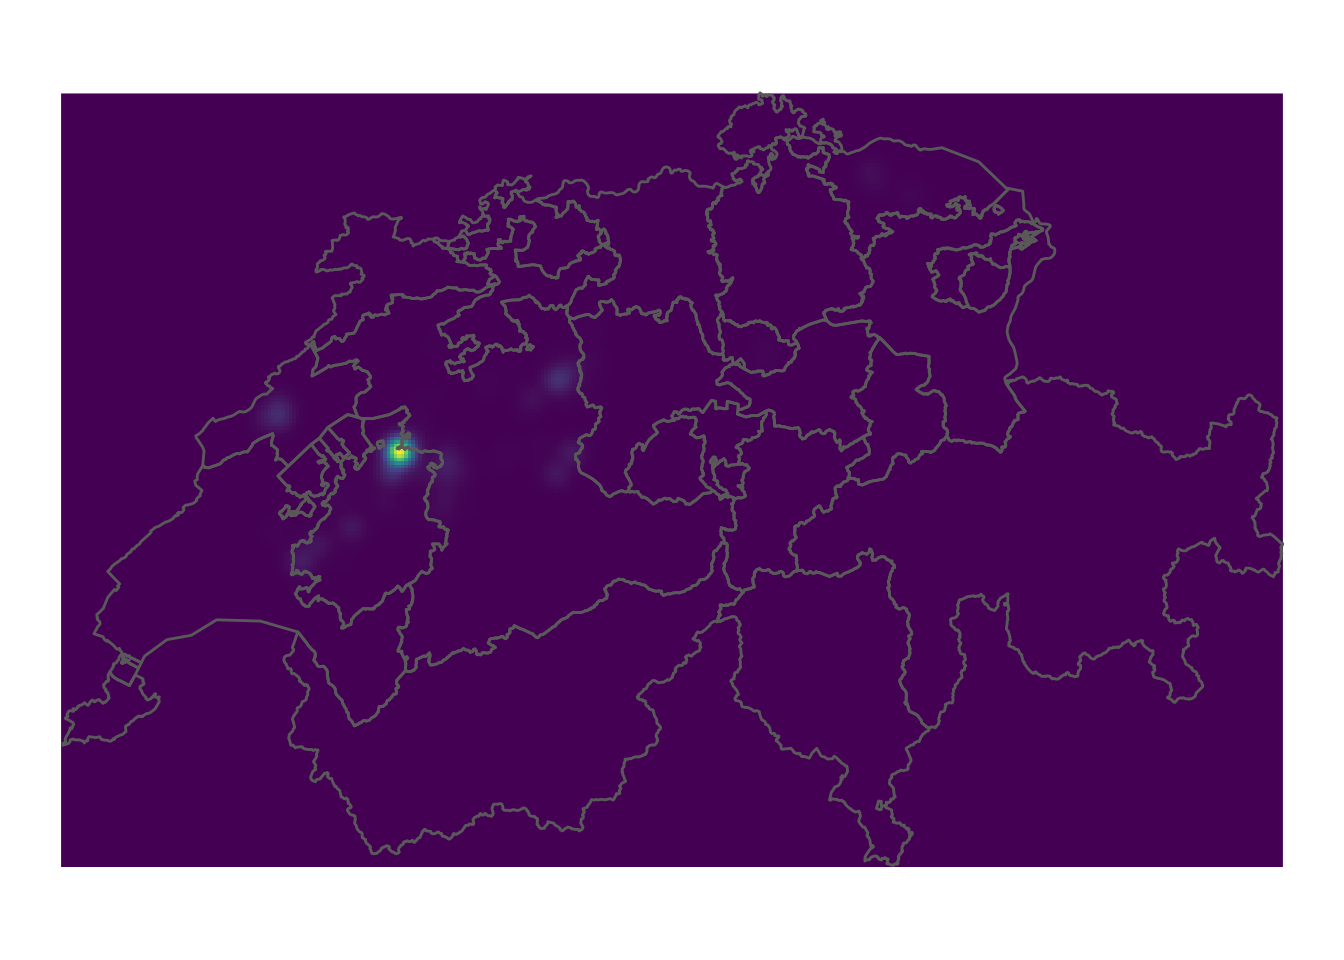
\includegraphics{_main_files/figure-latex/unnamed-chunk-52-1.pdf}

Nun schauen wir uns das plotten mit \texttt{ggplot2} an. Ein simpler Plot wie der in der vorherigen Aufgabe ist in \texttt{ggplot2} zugegebenermassen \emph{etwas} komplizierter. \texttt{ggplot2} wird aber rasch einfacher, wenn die Grafiken komplexer werden. Wir empfehlen deshalb stark, \texttt{ggplot2} zu verwenden.

Schau dir ein paar online Tutorials zu \texttt{ggplot2} an (siehe\footnote{Wickham and Grolemund (\protect\hyperlink{ref-wickham2017}{2017}), Kapitel 1 bzw. \url{http://r4ds.had.co.nz/data-visualisation.html} oder hier ein sehr schönes Video: \href{https://youtu.be/YxKr2a-Y1WE?t=1m40s}{Learn R: An Introduction to ggplot2}})
und reproduziere den obigen Plot mit \texttt{ggplot2}

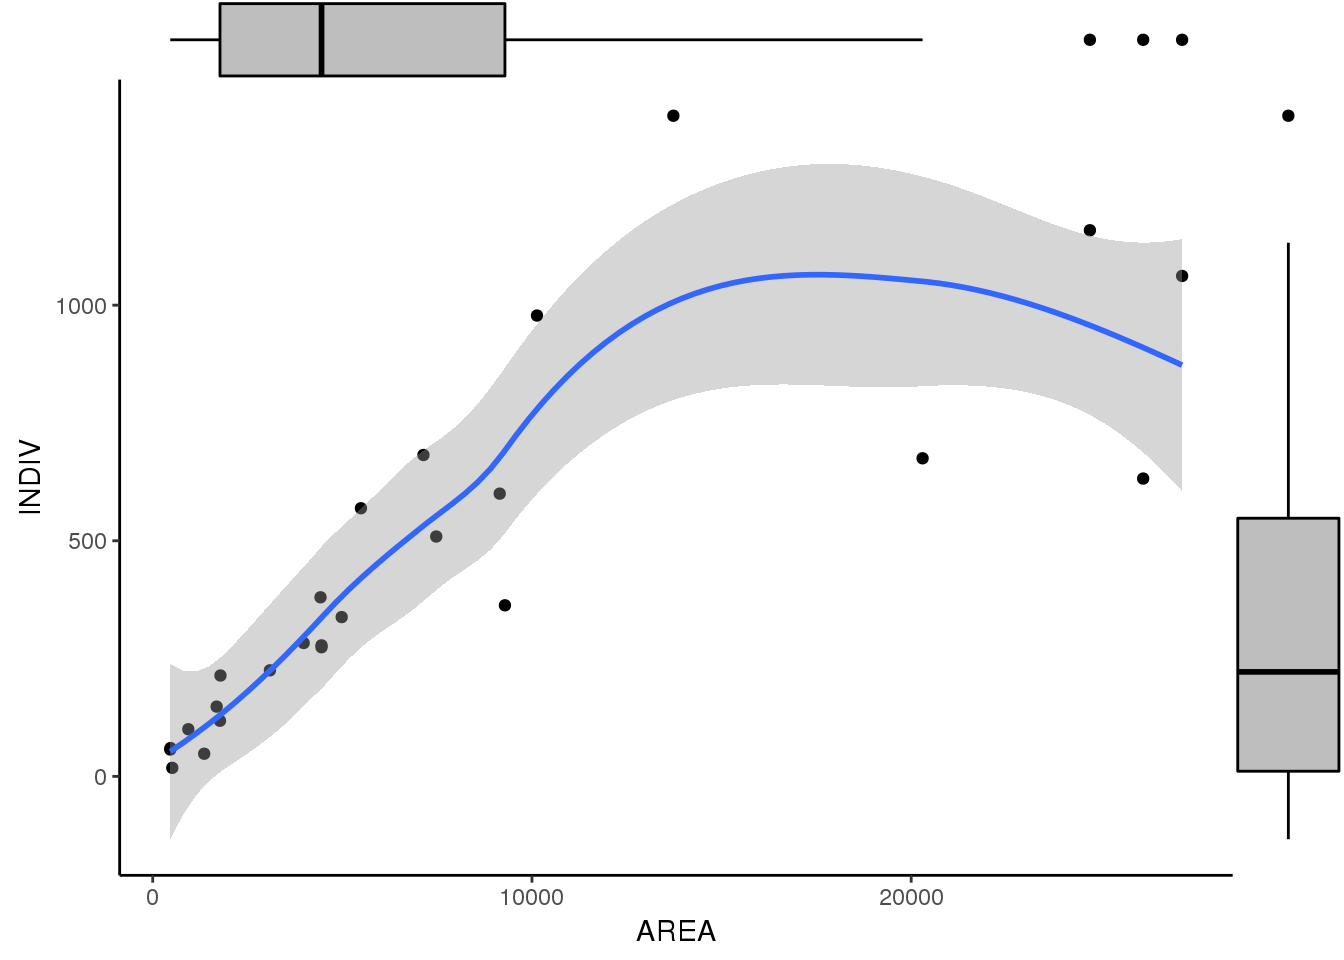
\includegraphics{_main_files/figure-latex/unnamed-chunk-53-1.pdf}

\hypertarget{aufgabe-2-1}{%
\subsection{Aufgabe 2}\label{aufgabe-2-1}}

Spiele mit Hilfe der erwähnten Tutorials mit dem Plot etwas rum. Versuche die x-/y-Achsen zu beschriften sowie einen Titel hinzu zu fügen.

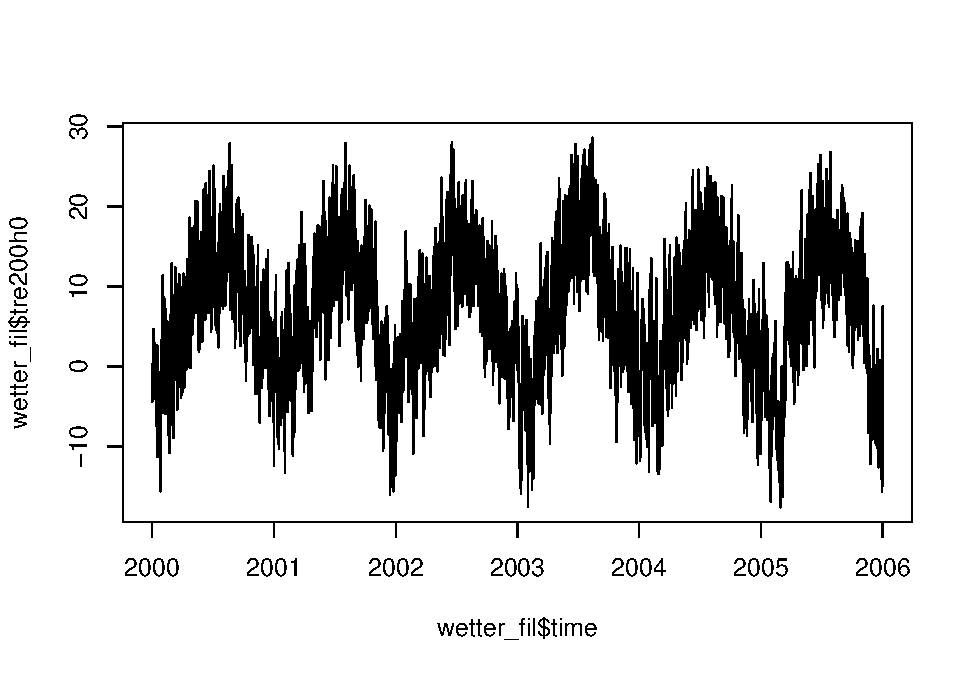
\includegraphics{_main_files/figure-latex/unnamed-chunk-54-1.pdf}

\hypertarget{aufgabe-3-1}{%
\subsection{Aufgabe 3}\label{aufgabe-3-1}}

Reduziere den x-Achsenausschnitt auf einen kleineren Zeitraum, beispielsweise einn beliebigen Monat. Verwende dazu \texttt{lims()} zusammen mit \texttt{as.POSIXct()} oder mache ein Subset von deinem Datensatz mit einer convenience-Variabel und \texttt{filter()}.

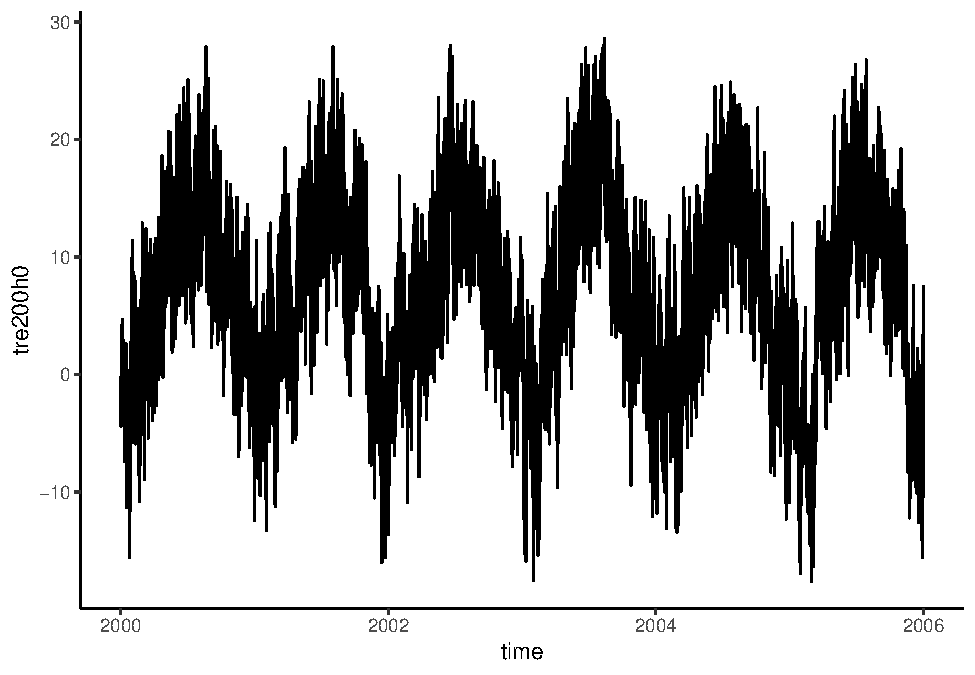
\includegraphics{_main_files/figure-latex/unnamed-chunk-55-1.pdf}

\hypertarget{prepro2-15.10.2019}{%
\chapter{PrePro2 (15.10.2019)}\label{prepro2-15.10.2019}}

Die Lerneinheit vermittelt zentralste Fertigkeiten zur Vorverarbeitung von strukturierten Daten in der umweltwissenschaftlichen Forschung: Datensätze verbinden (Joins) und umformen („reshape``, „split-apply-combine``). Im Anwendungskontext haben Daten selten von Anfang an diejenige Struktur, welche für die statistische Auswertung oder für die Informationsvisualisierung erforderlich wäre. In dieser Lerneinheit lernen die Studierenden die für diese oft zeitraubenden Preprocessing-Schritte notwendigen Konzepte und R-Werkzeuge kennen und kompetent anzuwenden.

\hypertarget{erganzungen-zu-prepro-1}{%
\section{Ergänzungen zu PrePro 1}\label{erganzungen-zu-prepro-1}}

\hypertarget{integer-mit-l}{%
\subsection{Integer mit ``L''}\label{integer-mit-l}}

In \texttt{R} kann eine Zahl mit dem Suffix ``L'' explizit als Integer spezifiziert werden.

\begin{Shaded}
\begin{Highlighting}[]
\KeywordTok{typeof}\NormalTok{(}\DecValTok{42}\NormalTok{)}
\CommentTok{## [1] "double"}
\KeywordTok{typeof}\NormalTok{(42L)}
\CommentTok{## [1] "integer"}
\end{Highlighting}
\end{Shaded}

Warum dazu der Buchstabe ``L'' verwendet wird ist nirgends offiziell Dokumentiert (zumindest haben wir nichts gefunden). Die gängigste Meinung, die auch \href{https://hypatia.math.ethz.ch/pipermail/r-devel/2017-June/074467.html}{von renommierten R-Profis vertreten wird} ist, dass damit \texttt{Long\ integer} abgekürzt wird.

\hypertarget{arbeiten-mit-rstudio-project}{%
\subsection{Arbeiten mit RStudio ``Project''}\label{arbeiten-mit-rstudio-project}}

Wir empfehlen die Verwendung von ``Projects'' innerhalb von RStudio. RStudio legt für jedes Projekt dann einen Ordner an, in welches die Projekt-Datei abgelegt wird (Dateiendung .Rproj). Sollen innerhalb des Projekts dann R-Skripts geladen oder erzeugt werden, werden diese dann auch im angelegten Ordner abgelegt. Mehr zu RStudio Projects findet ihr \href{https://support.rstudio.com/hc/en-us/articles/200526207-Using-Projects}{hier}.

Das Verwenden von Projects bringt verschiedene Vorteile, wie zum Beispiel:

\begin{itemize}
\tightlist
\item
  Festlegen der Working Directory ohne die Verwendung des expliziten Pfades (\texttt{setwd()}). Das ist sinnvoll, da sich dieser Pfad ändern kann (Zusammenarbeit mit anderen Usern, Ausführung des Scripts zu einem späteren Zeitpunkt)
\item
  Automatisches Zwischenspeichern geöffneter Scripts und Wiederherstellung der geöffneten Scripts bei der nächsten Session
\item
  Festlegen verschiedener projektspezifischer Optionen
\item
  Verwendung von Versionsverwaltungssystemen (Github oder SVN)
\end{itemize}

\hypertarget{arbeiten-mit-factors}{%
\subsection{\texorpdfstring{Arbeiten mit \texttt{factors}}{Arbeiten mit factors}}\label{arbeiten-mit-factors}}

Wie bereits angedeutet, ist das Arbeiten mit \texttt{factors} etwas gewöhnungsbedürftig. Wir gehen hier auf ein paar Stolpersteine ein.

\begin{Shaded}
\begin{Highlighting}[]
\NormalTok{zahlen <-}\StringTok{ }\KeywordTok{factor}\NormalTok{(}\KeywordTok{c}\NormalTok{(}\StringTok{"null"}\NormalTok{,}\StringTok{"eins"}\NormalTok{,}\StringTok{"zwei"}\NormalTok{,}\StringTok{"drei"}\NormalTok{))}

\NormalTok{zahlen}
\CommentTok{## [1] null eins zwei drei}
\CommentTok{## Levels: drei eins null zwei}
\end{Highlighting}
\end{Shaded}

Offensichtlich sollten diese \texttt{factors} geordnet sein, R weiss davon aber nichts. Eine Ordnung kann man mit dem Befehl \texttt{ordered\ =\ T} festlegen.

Beachtet: \texttt{ordered\ =\ T} kann nur bei der Funktion \texttt{factor()} spezifiziert werden, nicht bei \texttt{as.factor()}. Ansonsten sind \texttt{factor()} und \texttt{as.factor()} sehr ähnlich.

\begin{Shaded}
\begin{Highlighting}[]
\NormalTok{zahlen <-}\StringTok{ }\KeywordTok{factor}\NormalTok{(zahlen,}\DataTypeTok{ordered =}\NormalTok{ T)}

\NormalTok{zahlen}
\CommentTok{## [1] null eins zwei drei}
\CommentTok{## Levels: drei < eins < null < zwei}
\end{Highlighting}
\end{Shaded}

Beachtet das ``\textless{}''-Zeichen zwischen den Levels. Die Zahlen werden nicht in der korrekten Reihenfolge, sondern Alphabetisch geordnet. Die richtige Reihenfolge kann man mit \texttt{levels\ =} festlegen.

\begin{Shaded}
\begin{Highlighting}[]
\NormalTok{zahlen <-}\StringTok{ }\KeywordTok{factor}\NormalTok{(zahlen,}\DataTypeTok{ordered =}\NormalTok{ T,}\DataTypeTok{levels =} \KeywordTok{c}\NormalTok{(}\StringTok{"null"}\NormalTok{,}\StringTok{"eins"}\NormalTok{,}\StringTok{"zwei"}\NormalTok{,}\StringTok{"drei"}\NormalTok{,}\StringTok{"vier"}\NormalTok{))}

\NormalTok{zahlen}
\CommentTok{## [1] null eins zwei drei}
\CommentTok{## Levels: null < eins < zwei < drei < vier}
\end{Highlighting}
\end{Shaded}

Wie auch schon erwähnt werden \texttt{factors} als \texttt{character} Vektor dargestellt, aber als Integers gespeichert. Das führt zu einem scheinbaren Wiederspruch wenn man den Datentyp auf unterschiedliche Weise abfragt.

\begin{Shaded}
\begin{Highlighting}[]
\KeywordTok{typeof}\NormalTok{(zahlen)}
\CommentTok{## [1] "integer"}

\KeywordTok{is.integer}\NormalTok{(zahlen)}
\CommentTok{## [1] FALSE}
\end{Highlighting}
\end{Shaded}

Mit \texttt{typeof()} wird eben diese Form der Speicherung abgefragt und deshalb mit \texttt{integer} beantwortet. Da es sich aber nicht um einen eigentlichen Integer Vektor handelt, wird die Frage \texttt{is.integer()} mit \texttt{FALSE} beantwortet. Das ist etwas verwirrend, beruht aber darauf, dass die beiden Funktionen die Frage von unterschiedlichen Perspektiven beantworten. In diesem Fall schafft \texttt{class()} Klarheit:

\begin{Shaded}
\begin{Highlighting}[]
\KeywordTok{class}\NormalTok{(zahlen)}
\CommentTok{## [1] "ordered" "factor"}
\end{Highlighting}
\end{Shaded}

Wirklich verwirrend wird es, wenn \texttt{factors} in numeric umgewandelt werden sollen.

\begin{Shaded}
\begin{Highlighting}[]
\NormalTok{zahlen}
\CommentTok{## [1] null eins zwei drei}
\CommentTok{## Levels: null < eins < zwei < drei < vier}
\KeywordTok{as.integer}\NormalTok{(zahlen)}
\CommentTok{## [1] 1 2 3 4}
\end{Highlighting}
\end{Shaded}

Das die Übersetzung der auf Deutsch ausgeschriebenen Nummern in nummerische Zahlen nicht funktionieren würde, war ja klar. Weniger klar ist es jedoch, wenn die \texttt{factors} bereits aus nummerischen Zahlen bestehen.

\begin{Shaded}
\begin{Highlighting}[]
\NormalTok{zahlen2 <-}\StringTok{ }\KeywordTok{factor}\NormalTok{(}\KeywordTok{c}\NormalTok{(}\StringTok{"3"}\NormalTok{,}\StringTok{"2"}\NormalTok{,}\StringTok{"1"}\NormalTok{,}\StringTok{"0"}\NormalTok{))}

\KeywordTok{as.integer}\NormalTok{(zahlen2)}
\CommentTok{## [1] 4 3 2 1}
\end{Highlighting}
\end{Shaded}

In diesem Fall müssen die \texttt{factors} erstmals in \texttt{character} umgewandelt werden.

\begin{Shaded}
\begin{Highlighting}[]
\NormalTok{zahlen2 <-}\StringTok{ }\KeywordTok{factor}\NormalTok{(}\KeywordTok{c}\NormalTok{(}\StringTok{"3"}\NormalTok{,}\StringTok{"2"}\NormalTok{,}\StringTok{"1"}\NormalTok{,}\StringTok{"0"}\NormalTok{))}

\KeywordTok{as.integer}\NormalTok{(}\KeywordTok{as.character}\NormalTok{(zahlen2))}
\CommentTok{## [1] 3 2 1 0}
\end{Highlighting}
\end{Shaded}

\hypertarget{heikle-annahmen---bessere-alternativen}{%
\subsection{Heikle Annahmen - bessere Alternativen}\label{heikle-annahmen---bessere-alternativen}}

Aus oben beschriebenen Grund ist es auch problematisch, dass \texttt{data.frame()} sowie alle \texttt{read.*} Funktionen (\texttt{read.table}, \texttt{read.csv} etc) immer davon ausgehen, dass \texttt{Strings} als \texttt{factors} interpretiert werden sollten. Es gibt in Base R einige Funktionen, welche Annahmen treffen die problematisch sein können. Ein weiteres Beispiel ist die Annahme der Zeitzone und Verwendung von Sommerzeit bei \texttt{as.POSIXct()}.

Oft gibt es dafür im Tidyverse alternative Funktionen, in denen diese Probleme besser gelöst sind. Wir empfehlen, wenn immer Möglich die Tidyverse-Alternativen zu verwenden. Beispiele:

\begin{itemize}
\tightlist
\item
  \texttt{data\_frame()} statt \texttt{data.frame()}
\item
  \texttt{read\_*} statt \texttt{read.*}
\item
  \texttt{parse\_datetime} statt \texttt{as.POSIXct()}
\end{itemize}

Beim Import von Daten kann es sinnvoll sein, die Datentypen der Spalten bereits \emph{im Importbefehl} zu spezifizieren. So vermeidet man die anschliessende Typumwandlung und die damit verbundenen Fehlerquellen. Zudem wird der Importprozess beschleunigt, da R keine Zeit daran verschwenden muss die Datentypen (aufgrund der ersten 1000 Zeilen) zu erraten.

\begin{Shaded}
\begin{Highlighting}[]

\KeywordTok{library}\NormalTok{(tidyverse)}

\NormalTok{df1 <-}\StringTok{ }\KeywordTok{read_table}\NormalTok{(}\StringTok{"09_PrePro1/data/order_52252_data.txt"}\NormalTok{,}
                  \DataTypeTok{col_types =} \KeywordTok{list}\NormalTok{(}
                    \KeywordTok{col_character}\NormalTok{(),                  }\CommentTok{# Macht aus der 1.Spalte ein character}
                    \KeywordTok{col_datetime}\NormalTok{(}\DataTypeTok{format =} \StringTok{"%Y%m%d%H"}\NormalTok{),}\CommentTok{# Macht aus der 2.Spalte ein POSIXct}
                    \KeywordTok{col_double}\NormalTok{()                      }\CommentTok{# Macht aus der 3.Spalte ein double}
\NormalTok{                    )}
\NormalTok{                  )}

\NormalTok{df1}
\CommentTok{## # A tibble: 1,262,615 x 3}
\CommentTok{##    stn   time                tre200h0}
\CommentTok{##    <chr> <dttm>                 <dbl>}
\CommentTok{##  1 ABO   2000-01-01 00:00:00     -2.6}
\CommentTok{##  2 ABO   2000-01-01 01:00:00     -2.5}
\CommentTok{##  3 ABO   2000-01-01 02:00:00     -3.1}
\CommentTok{##  4 ABO   2000-01-01 03:00:00     -2.4}
\CommentTok{##  5 ABO   2000-01-01 04:00:00     -2.5}
\CommentTok{##  6 ABO   2000-01-01 05:00:00     -3  }
\CommentTok{##  7 ABO   2000-01-01 06:00:00     -3.7}
\CommentTok{##  8 ABO   2000-01-01 07:00:00     -4.4}
\CommentTok{##  9 ABO   2000-01-01 08:00:00     -4.1}
\CommentTok{## 10 ABO   2000-01-01 09:00:00     -4.1}
\CommentTok{## # ... with 1,262,605 more rows}

\NormalTok{df1 <-}\StringTok{ }\KeywordTok{read_table}\NormalTok{(}\StringTok{"09_PrePro1/data/order_52252_data.txt"}\NormalTok{,}
                  \DataTypeTok{col_types =} \KeywordTok{list}\NormalTok{(}
                    \KeywordTok{col_factor}\NormalTok{(}\DataTypeTok{levels =} \OtherTok{NULL}\NormalTok{),        }\CommentTok{# Macht aus der 1.Spalte ein factor}
                    \KeywordTok{col_datetime}\NormalTok{(}\DataTypeTok{format =} \StringTok{"%Y%m%d%H"}\NormalTok{),}\CommentTok{# Macht aus der 2.Spalte ein POSIXct}
                    \KeywordTok{col_double}\NormalTok{()                      }\CommentTok{# Macht aus der 3.Spalte ein double}
\NormalTok{                    )}
\NormalTok{                  )}


\NormalTok{df1}
\CommentTok{## # A tibble: 1,262,615 x 3}
\CommentTok{##    stn   time                tre200h0}
\CommentTok{##    <fct> <dttm>                 <dbl>}
\CommentTok{##  1 ABO   2000-01-01 00:00:00     -2.6}
\CommentTok{##  2 ABO   2000-01-01 01:00:00     -2.5}
\CommentTok{##  3 ABO   2000-01-01 02:00:00     -3.1}
\CommentTok{##  4 ABO   2000-01-01 03:00:00     -2.4}
\CommentTok{##  5 ABO   2000-01-01 04:00:00     -2.5}
\CommentTok{##  6 ABO   2000-01-01 05:00:00     -3  }
\CommentTok{##  7 ABO   2000-01-01 06:00:00     -3.7}
\CommentTok{##  8 ABO   2000-01-01 07:00:00     -4.4}
\CommentTok{##  9 ABO   2000-01-01 08:00:00     -4.1}
\CommentTok{## 10 ABO   2000-01-01 09:00:00     -4.1}
\CommentTok{## # ... with 1,262,605 more rows}
\end{Highlighting}
\end{Shaded}

\hypertarget{demo-tidyverse}{%
\section{\texorpdfstring{Demo: \texttt{tidyverse}}{Demo: tidyverse}}\label{demo-tidyverse}}

\href{10_PrePro2/RFiles/Demo_Tidyverse.R}{Demoscript als Download}

Hier möchten wir euch mit einer Sammlung von Tools vertraut machen, die spezifisch für das Daten prozessieren in Data Science entwickelt wurden. Der Prozess und das Modell ist hier\footnote{\url{http://r4ds.had.co.nz/introduction.html\#}} schön beschrieben.
Die Sammlung von Tools wird unter dem Namen \href{https://www.tidyverse.org/}{tidyverse} vertrieben, welches wir ja schon zu Beginn der ersten Übung installiert und geladen haben. Die Tools erleichtern den Umgang mit Daten ungeheuer und haben sich mittlerweile zu einem ``must have'' im Umgang mit Daten in R entwickelt.

Wir können Euch nicht sämtliche Möglichkeiten von tidyverse zeigen. Wir fokussieren uns deshalb auf einzelne Komponenten\footnote{\texttt{dplyr,\ ggplot2,\ tidyr,\ stringr,\ magrittr,\ lubridate}} und zeigen ein paar Funktionalitäten, die wir oft verwenden und Euch ggf. noch nicht bekannt sind. Wer sich vertieft mit dem Thema auseinandersetzen möchte, der sollte sich unbedingt das Buch Wickham and Grolemund (\protect\hyperlink{ref-wickham2017}{2017}) beschaffen. Eine umfangreiche, aber nicht ganz vollständige Version gibt es online\footnote{\url{http://r4ds.had.co.nz/}}, das vollständige eBook kann über die Bibliothek bezogen werden\footnote{\url{https://ebookcentral.proquest.com/lib/zhaw/detail.action?docID=4770093}}.

\hypertarget{split-apply-combine}{%
\subsection{Split-Apply-Combine}\label{split-apply-combine}}

\hypertarget{packete-laden}{%
\subsubsection{Packete laden}\label{packete-laden}}

\begin{Shaded}
\begin{Highlighting}[]
\KeywordTok{library}\NormalTok{(tidyverse)}
\end{Highlighting}
\end{Shaded}

Mit \texttt{library(tidyverse)} werden nicht alle Packete geladen, die mit \texttt{install.packages(tidyverse)} intalliert wurden (\href{https://community.rstudio.com/t/which-packages-get-loaded/298}{warum?}). Unter anderem muss \texttt{lubridate} noch separat geladen werden:

\begin{Shaded}
\begin{Highlighting}[]
\KeywordTok{library}\NormalTok{(lubridate) }
\end{Highlighting}
\end{Shaded}

\hypertarget{daten-laden}{%
\subsubsection{Daten Laden}\label{daten-laden}}

Wir laden die Wetterdaten von der letzten Übung.

\begin{Shaded}
\begin{Highlighting}[]

\NormalTok{wetter <-}\StringTok{ }\KeywordTok{read_table}\NormalTok{(}\StringTok{"09_PrePro1/data/order_52252_data.txt"}\NormalTok{,}
                  \DataTypeTok{col_types =} \KeywordTok{list}\NormalTok{(}
                    \KeywordTok{col_factor}\NormalTok{(}\DataTypeTok{levels =} \OtherTok{NULL}\NormalTok{),    }
                    \KeywordTok{col_datetime}\NormalTok{(}\DataTypeTok{format =} \StringTok{"%Y%m%d%H"}\NormalTok{),}
                    \KeywordTok{col_double}\NormalTok{()}
\NormalTok{                    )}
\NormalTok{                  )}
\end{Highlighting}
\end{Shaded}

\hypertarget{kennwerte-berechnen}{%
\subsubsection{Kennwerte berechnen}\label{kennwerte-berechnen}}

Wir möchten den Mittelwert aller gemessenen Temperaturwerte berechnen. Dazu könnten wir folgenden Befehl verwenden:

\begin{Shaded}
\begin{Highlighting}[]
\KeywordTok{mean}\NormalTok{(wetter}\OperatorTok{$}\NormalTok{tre200h0, }\DataTypeTok{na.rm =}\NormalTok{ T) }
\CommentTok{## [1] 8.962106}
\end{Highlighting}
\end{Shaded}

Die Option \texttt{na.rm\ =\ T} bedeutet, dass NA Werte von der Berechnung ausgeschlossen werden sollen.

Mit der selben Herangehensweise können diverse Werte berechnet werden (z.B. das Maximum (\texttt{max()}), Minimum (\texttt{min()}), Median (\texttt{median()}) u.v.m.).

Diese Herangehensweise funktioniert nur dann gut, wenn wir die Kennwerte über \emph{alle} Beobachtungen (Zeilen) für eine Variable (Spalte) berechnen wollen. Sobald wir die Beobachtungen gruppieren wollen, wird es schwierig. Zum Beispiel, wenn wir die durchschnittliche Temperatur \emph{pro Jahr} berechnen wollen.

\hypertarget{convenience-variablen}{%
\subsubsection{Convenience Variablen}\label{convenience-variablen}}

Um diese Aufgabe zu lösen, muss zuerst das ``Jahr'' berechne werden (das Jahr ist die \emph{convenience variabel}). Hierfür brauchen wir die Funktion \texttt{year()} (von \texttt{lubridate}).

Nun kann kann die \textbf{convenience Variable} ``Jahr'' erstellt werden. Ohne \texttt{dpylr} wird eine neue Spalte wird folgendermassen hinzugefügt.

\begin{Shaded}
\begin{Highlighting}[]
\NormalTok{wetter}\OperatorTok{$}\NormalTok{year <-}\StringTok{ }\KeywordTok{year}\NormalTok{(wetter}\OperatorTok{$}\NormalTok{time)}
\end{Highlighting}
\end{Shaded}

Mit \texttt{dplyr} (siehe\footnote{Wickham and Grolemund (\protect\hyperlink{ref-wickham2017}{2017}), Kapitel 10 / \url{http://r4ds.had.co.nz/transform.html}}) sieht der gleiche Befehl folgendermassen aus:

\begin{Shaded}
\begin{Highlighting}[]
\NormalTok{wetter <-}\StringTok{ }\KeywordTok{mutate}\NormalTok{(wetter,}\DataTypeTok{year =} \KeywordTok{year}\NormalTok{(time))}
\end{Highlighting}
\end{Shaded}

Der grosse Vorteil von \texttt{dplyr} ist an dieser Stelle noch nicht ersichtlich. Dieser wird aber später klar.

\hypertarget{kennwerte-nach-gruppen-berechnen}{%
\subsubsection{Kennwerte nach Gruppen berechnen}\label{kennwerte-nach-gruppen-berechnen}}

Jetzt kann man die \texttt{data.frame} mithilfe der Spalte ``Jahr'' filtern.

\begin{Shaded}
\begin{Highlighting}[]
\KeywordTok{mean}\NormalTok{(wetter}\OperatorTok{$}\NormalTok{tre200h0[wetter}\OperatorTok{$}\NormalTok{year }\OperatorTok{==}\StringTok{ }\DecValTok{2000}\NormalTok{], }\DataTypeTok{na.rm =}\NormalTok{ T)}
\CommentTok{## [1] 9.281542}
\end{Highlighting}
\end{Shaded}

Dies müssen wir pro Jahr wiederholen, was natürlich sehr umständlich ist, v.a. wenn man eine Vielzahl an Gruppen hat (z.B. Kalenderwochen statt Jahre). Deshalb nutzen wir das package \texttt{dplyr}. Damit geht die Aufgabe (Temperaturmittel pro Jahr berechnen) folgendermassen:

\begin{Shaded}
\begin{Highlighting}[]
\KeywordTok{summarise}\NormalTok{(}\KeywordTok{group_by}\NormalTok{(wetter,year),}\DataTypeTok{temp_mittel =} \KeywordTok{mean}\NormalTok{(tre200h0, }\DataTypeTok{na.rm =}\NormalTok{ T))}
\CommentTok{## # A tibble: 7 x 2}
\CommentTok{##    year temp_mittel}
\CommentTok{##   <dbl>       <dbl>}
\CommentTok{## 1  2000        9.28}
\CommentTok{## 2  2001        8.76}
\CommentTok{## 3  2002        9.30}
\CommentTok{## 4  2003        9.48}
\CommentTok{## 5  2004        8.64}
\CommentTok{## 6  2005        8.31}
\CommentTok{## 7    NA      NaN}
\end{Highlighting}
\end{Shaded}

\hypertarget{verketten-vs.verschachteln}{%
\subsubsection{Verketten vs.~verschachteln}\label{verketten-vs.verschachteln}}

Auf Deutsch übersetzt heisst die obige Operation folgendermassen:

\begin{enumerate}
\def\labelenumi{\arabic{enumi})}
\tightlist
\item
  nimm den Datensatz \texttt{wetter}
\item
  Bilde Gruppen pro Jahr (\texttt{group\_by(wetter,year)})
\item
  Berechne das Temperaturmittel (\texttt{mean(tre200h0)})
\end{enumerate}

Diese Übersetzung \texttt{R}-\textgreater{} Deutsch unterscheidet sich vor allem darin, dass die Operation auf Deutsch \emph{verkettet} ausgesprochen wird (Operation 1-\textgreater{}2-\textgreater{}3) während der Computer \emph{verschachtelt} liest 3(2(1)). Um \texttt{R} näher an die gesprochene Sprache zu bringen, kann man den \texttt{\%\textgreater{}\%}-Operator verwenden (siehe\footnote{Wickham and Grolemund (\protect\hyperlink{ref-wickham2017}{2017}), Kapitel 14 / \url{http://r4ds.had.co.nz/pipes.html}}).

\begin{Shaded}
\begin{Highlighting}[]

\KeywordTok{summarise}\NormalTok{(}\KeywordTok{group_by}\NormalTok{(wetter,year),}\DataTypeTok{temp_mittel =} \KeywordTok{mean}\NormalTok{(tre200h0))}

\CommentTok{# wird zu:}

\NormalTok{wetter }\OperatorTok\StringTok{                                }\CommentTok{#1) nimm den Datensatz "wetter"}
\StringTok{  }\KeywordTok{group_by}\NormalTok{(year) }\OperatorTok\StringTok{                      }\CommentTok{#2) Bilde Gruppen pro Jahr}
\StringTok{  }\KeywordTok{summarise}\NormalTok{(}\DataTypeTok{temp_mittel =} \KeywordTok{mean}\NormalTok{(tre200h0)) }\CommentTok{#3) berechne das Temperaturmittel }
\end{Highlighting}
\end{Shaded}

Dieses Verketten mittels \texttt{\%\textgreater{}\%} macht den Code einiges schreib- und leserfreundlicher, und wir werden ihn in den nachfolgenden Übungen verwenden. Dabei handelt es sich um das package \texttt{magrittr}, welches mit \texttt{tidyverse} mitgeliefert wird.

Zu \texttt{dplyr} und \texttt{magrittr}gibt es etliche Tutorials online (siehe\footnote{Wickham and Grolemund (\protect\hyperlink{ref-wickham2017}{2017}), Kapitel 10 / \url{http://r4ds.had.co.nz/transform.html}, oder \href{https://youtu.be/jWjqLW-u3hc}{Hands-on dplyr tutorial..}}), deshalb werden wir diese Tools nicht in allen Details erläutern. Nur noch folgenden wichtigen Unterschied zu zwei wichtigen Funktionen in \texttt{dpylr}: \texttt{mutate()} und \texttt{summarise()}.

\begin{itemize}
\tightlist
\item
  \texttt{summarise()} fasst einen Datensatz zusammen. Dabei reduziert sich die Anzahl Beobachtungen (Zeilen) auf die Anzahl Gruppen (z.B. eine zusammengefasste Beobachtung (Zeile) pro Jahr). Zudem reduziert sich die Anzahl Variablen (Spalten) auf diejenigen, die in der ``summarise'' Funktion spezifiziert wurde (z.B. \texttt{temp\_mittel}).
\item
  mit \texttt{mutate} wird ein \texttt{data.frame} vom Umfang her belassen, es werden lediglich \emph{zusätzliche} Variablen (Spalten) hinzugefügt (siehe Beispiel unten).
\end{itemize}

\begin{Shaded}
\begin{Highlighting}[]
\CommentTok{# Maximal und minimal Temperatur pro Kalenderwoche}
\NormalTok{wetter }\OperatorTok\StringTok{                              }\CommentTok{#1) nimm den Datensatz "wetter"}
\StringTok{  }\KeywordTok{filter}\NormalTok{(stn }\OperatorTok{==}\StringTok{ "ABO"}\NormalTok{) }\OperatorTok\StringTok{              }\CommentTok{#2) filter auf Station namnes "ABO"}
\StringTok{  }\KeywordTok{mutate}\NormalTok{(}\DataTypeTok{kw =} \KeywordTok{week}\NormalTok{(time)) }\OperatorTok\StringTok{       }\CommentTok{#3) erstelle eine neue Spalte "kw"}
\StringTok{  }\KeywordTok{group_by}\NormalTok{(kw) }\OperatorTok\StringTok{                      }\CommentTok{#4) Nutze die neue Spalte um Guppen zu bilden}
\StringTok{  }\KeywordTok{summarise}\NormalTok{(}
    \DataTypeTok{temp_max =} \KeywordTok{max}\NormalTok{(tre200h0, }\DataTypeTok{na.rm =}\NormalTok{ T),}\CommentTok{#5) Berechne das Maximum }
    \DataTypeTok{temp_min =} \KeywordTok{min}\NormalTok{(tre200h0, }\DataTypeTok{na.rm =}\NormalTok{ T) }\CommentTok{#6) Berechne das Minimum}
\NormalTok{    )   }
\CommentTok{## # A tibble: 53 x 3}
\CommentTok{##       kw temp_max temp_min}
\CommentTok{##    <dbl>    <dbl>    <dbl>}
\CommentTok{##  1     1     11.4    -15.2}
\CommentTok{##  2     2     12.9    -15.9}
\CommentTok{##  3     3      8.2    -11.3}
\CommentTok{##  4     4      9.6    -15.9}
\CommentTok{##  5     5     16.9    -17.5}
\CommentTok{##  6     6     13.5    -13.1}
\CommentTok{##  7     7     12.9    -15.4}
\CommentTok{##  8     8     11      -14.4}
\CommentTok{##  9     9     12.9    -17.6}
\CommentTok{## 10    10     15.4    -16.3}
\CommentTok{## # ... with 43 more rows}
\end{Highlighting}
\end{Shaded}

\hypertarget{resultate-plotten}{%
\subsubsection{Resultate plotten}\label{resultate-plotten}}

Mit diesen Tools können wir nun auch eine neue Grafik plotten, ähnlich wie in der Übung 1. Dafür müssen wir die ganzen Operationen aber zuerst in einer Variabel speichern (bis jetzt hat R zwar alles schön berechnet, aber uns nur auf die Konsole ausgegeben).

\begin{Shaded}
\begin{Highlighting}[]

\NormalTok{wetter_sry <-}\StringTok{ }\NormalTok{wetter }\OperatorTok\StringTok{                              }
\StringTok{  }\KeywordTok{mutate}\NormalTok{(}
    \DataTypeTok{kw =} \KeywordTok{week}\NormalTok{(time)}
\NormalTok{    ) }\OperatorTok
\StringTok{  }\KeywordTok{filter}\NormalTok{(stn }\OperatorTok{==}\StringTok{ "ABO"}\NormalTok{) }\OperatorTok
\StringTok{  }\KeywordTok{group_by}\NormalTok{(kw) }\OperatorTok\StringTok{                      }
\StringTok{  }\KeywordTok{summarise}\NormalTok{(}
    \DataTypeTok{temp_max =} \KeywordTok{max}\NormalTok{(tre200h0),               }
    \DataTypeTok{temp_min =} \KeywordTok{min}\NormalTok{(tre200h0),}
    \DataTypeTok{temp_mean =} \KeywordTok{mean}\NormalTok{(tre200h0)}
\NormalTok{    )  }
\end{Highlighting}
\end{Shaded}

Dieses Mal plotten wir nur mit \texttt{ggplot2} (siehe\footnote{Wickham and Grolemund (\protect\hyperlink{ref-wickham2017}{2017}), Kapitel 1 / \url{http://r4ds.had.co.nz/data-visualisation.html} oder hier ein sehr schönes Video: \href{https://youtu.be/YxKr2a-Y1WE?t=1m40s}{Learn R: An Introduction to ggplot2}})

\begin{Shaded}
\begin{Highlighting}[]

\KeywordTok{ggplot}\NormalTok{() }\OperatorTok{+}
\StringTok{  }\KeywordTok{geom_line}\NormalTok{(}\DataTypeTok{data =}\NormalTok{ wetter_sry, }\KeywordTok{aes}\NormalTok{(kw,temp_max), }\DataTypeTok{colour =} \StringTok{"yellow"}\NormalTok{) }\OperatorTok{+}
\StringTok{  }\KeywordTok{geom_line}\NormalTok{(}\DataTypeTok{data =}\NormalTok{ wetter_sry, }\KeywordTok{aes}\NormalTok{(kw,temp_mean), }\DataTypeTok{colour =} \StringTok{"pink"}\NormalTok{) }\OperatorTok{+}
\StringTok{  }\KeywordTok{geom_line}\NormalTok{(}\DataTypeTok{data =}\NormalTok{ wetter_sry, }\KeywordTok{aes}\NormalTok{(kw,temp_min), }\DataTypeTok{colour =} \StringTok{"black"}\NormalTok{) }\OperatorTok{+}
\StringTok{  }\KeywordTok{labs}\NormalTok{(}\DataTypeTok{y =} \StringTok{"temp"}\NormalTok{)}
\end{Highlighting}
\end{Shaded}

\includegraphics{_main_files/figure-latex/unnamed-chunk-82-1.pdf}

Das sieht schon mal gut aus. Nur, wir mussten pro Linie einen eigene Zeile schreiben (\texttt{geom\_line()}) und dieser eine Farbe zuweisen. Bei drei Werten ist das ja ok, aber wie sieht es denn aus wenn es Hunderte sind? Da hat ggplot natürlich eine Lösung, dafür müssen aber alle Werte in \emph{einer} Spalte daher kommen. Das ist ein häufiges Problem: Wir haben eine \emph{breite} Tabelle (viele Spalten), bräuchten aber eine \emph{lange} Tabelle (viele Zeilen).

\hypertarget{reshaping-data}{%
\subsection{Reshaping data}\label{reshaping-data}}

\hypertarget{breit---lang}{%
\subsubsection{Breit -\textgreater{} lang}\label{breit---lang}}

Da kommt \texttt{tidyverse} wieder ins Spiel. Die Umformung von Tabellen \emph{breit}-\textgreater{}\emph{lang} erfolgt mittels \texttt{tidyr}(siehe\footnote{\url{http://r4ds.had.co.nz/tidy-data.html\#gathering}}). Auch dieses package funktioniert wunderbar mit piping (\texttt{\%\textgreater{}\%}).

\begin{Shaded}
\begin{Highlighting}[]
\NormalTok{wetter_sry_long <-}\StringTok{ }\NormalTok{wetter_sry }\OperatorTok
\StringTok{  }\KeywordTok{gather}\NormalTok{(Key, Value, }\KeywordTok{c}\NormalTok{(temp_max,temp_min,temp_mean))}
\end{Highlighting}
\end{Shaded}

Im Befehl \texttt{gather()} braucht es drei Werte:

\begin{itemize}
\tightlist
\item
  beliebiger Name der neuen Variablen (Spalte) für die \emph{Schlüssel}: ``temp\_mean'', ``temp\_min''\ldots{} (ich verwenden den Namen: \texttt{Key})
\item
  beliebiger Name der neuen Variablen (Spalte) für die effektiven \emph{Werte}: 5°C, 10°C (ich verwenden den Namen: \texttt{Value})
\item
  Name der (bestehenden) Variablen (Spalten), die zusammen gefasst werden sollten: \texttt{(hier:\ temp\_max,temp\_min,temp\_mean})
\end{itemize}

Die ersten 6 Zeilen von \texttt{wetter\_sry}:

\begin{tabular}{r|r|r|r}
\hline
kw & temp\_max & temp\_min & temp\_mean\\
\hline
1 & 11.4 & -15.2 & -1.2593254\\
\hline
2 & 12.9 & -15.9 & -1.5572421\\
\hline
3 & 8.2 & -11.3 & -1.8832341\\
\hline
4 & 9.6 & -15.9 & -2.8375000\\
\hline
5 & 16.9 & -17.5 & -0.9789683\\
\hline
6 & 13.5 & -13.1 & 0.4392857\\
\hline
\end{tabular}

Die ersten 6 Zeilen von \texttt{wetter\_sry\_long}:

\begin{tabular}{r|l|r}
\hline
kw & Key & Value\\
\hline
1 & temp\_max & 11.400000\\
\hline
1 & temp\_min & -15.200000\\
\hline
1 & temp\_mean & -1.259325\\
\hline
2 & temp\_max & 12.900000\\
\hline
2 & temp\_min & -15.900000\\
\hline
2 & temp\_mean & -1.557242\\
\hline
\end{tabular}

Beachte: \texttt{wetter\_sry\_long} umfasst 159 Beobachtungen (Zeilen), das sind 3 mal soviel wie \texttt{wetter\_sry}, da wir ja drei Spalten zusammengefasst haben.

\begin{Shaded}
\begin{Highlighting}[]
\KeywordTok{nrow}\NormalTok{(wetter_sry)}
\CommentTok{## [1] 53}
\KeywordTok{nrow}\NormalTok{(wetter_sry_long)}
\CommentTok{## [1] 159}
\end{Highlighting}
\end{Shaded}

Statt die Variablen (Spalten) zu benennen, die zusammengefasst werden sollten, wäre es in unserem Fall einfacher, die Variablen (Spalten) zu benennen die \emph{nicht} zusammengefasst werden sollen (\texttt{kw}):

\begin{Shaded}
\begin{Highlighting}[]
\NormalTok{wetter_sry_long <-}\StringTok{ }\NormalTok{wetter_sry }\OperatorTok
\StringTok{  }\KeywordTok{gather}\NormalTok{(Key, Value, }\OperatorTok{-}\NormalTok{kw)}
\end{Highlighting}
\end{Shaded}

Nun können wir den obigen Plot viel einfacher erstellen:

\begin{Shaded}
\begin{Highlighting}[]
\KeywordTok{ggplot}\NormalTok{(wetter_sry_long, }\KeywordTok{aes}\NormalTok{(kw,Value, }\DataTypeTok{colour =}\NormalTok{ Key)) }\OperatorTok{+}
\StringTok{  }\KeywordTok{geom_line}\NormalTok{()}
\end{Highlighting}
\end{Shaded}

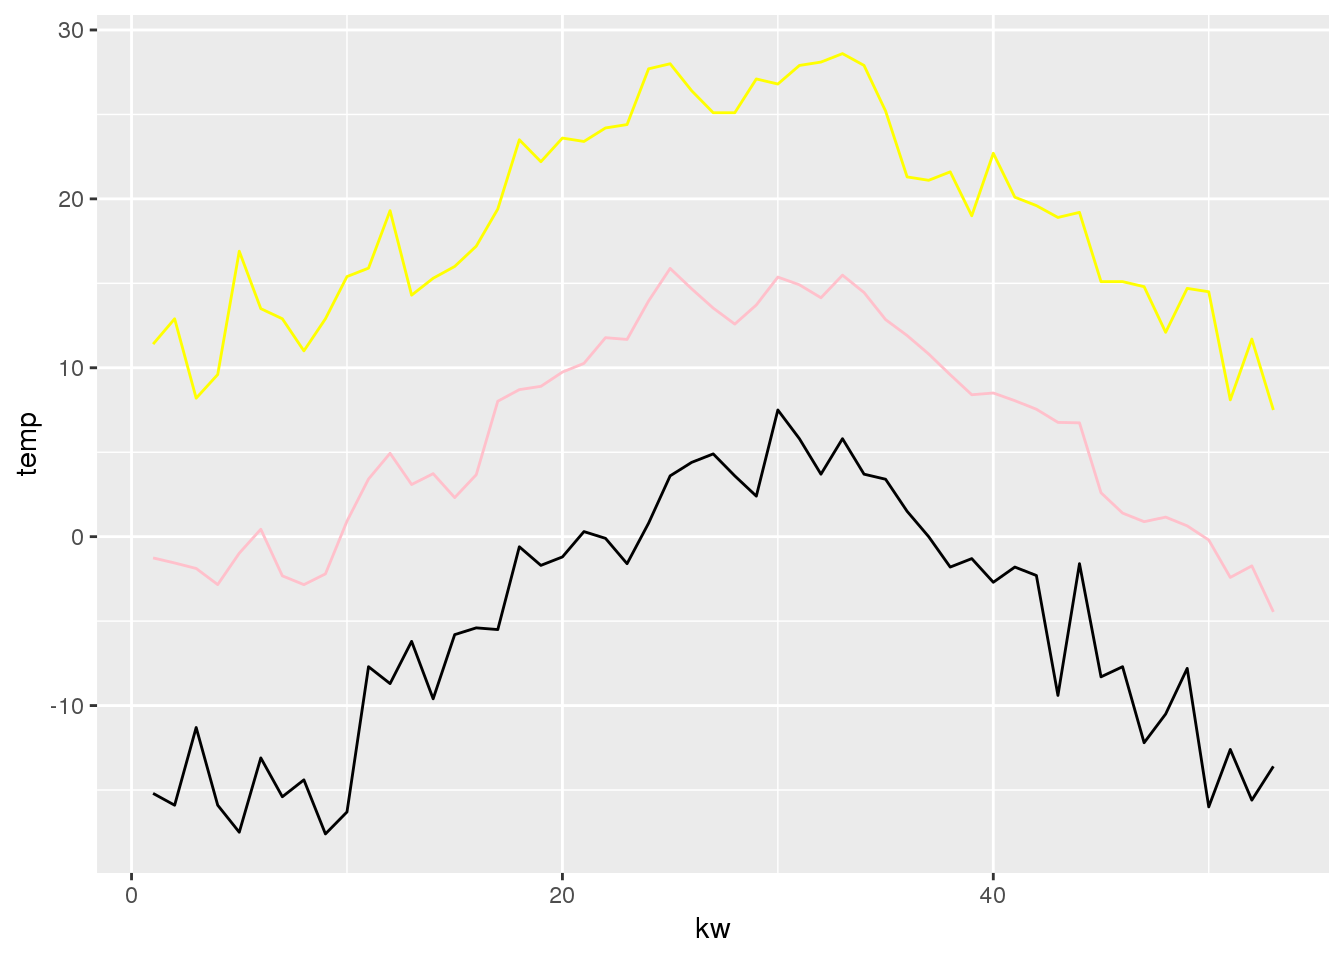
\includegraphics{_main_files/figure-latex/unnamed-chunk-88-1.pdf}

Beachtet, dass wir gegenüber dem letzten Plot \texttt{colour} nun \emph{innerhalb} von \texttt{aes()} festlegen und nicht mit einem expliziten Farbwert, sondern mit dem Verweis auf die Spalte \texttt{key}.

\hypertarget{lang---breit}{%
\subsubsection{Lang -\textgreater{} breit}\label{lang---breit}}

Um unsere \emph{lange} Tabelle wieder zurück in eine \emph{breite} zu überführen, brauchen wir lediglich einen Befehl (\texttt{spread}):

\begin{Shaded}
\begin{Highlighting}[]
\NormalTok{wetter_sry_long }\OperatorTok
\StringTok{  }\KeywordTok{spread}\NormalTok{(Key,Value)}
\CommentTok{## # A tibble: 53 x 4}
\CommentTok{##       kw temp_max temp_mean temp_min}
\CommentTok{##    <dbl>    <dbl>     <dbl>    <dbl>}
\CommentTok{##  1     1     11.4    -1.26     -15.2}
\CommentTok{##  2     2     12.9    -1.56     -15.9}
\CommentTok{##  3     3      8.2    -1.88     -11.3}
\CommentTok{##  4     4      9.6    -2.84     -15.9}
\CommentTok{##  5     5     16.9    -0.979    -17.5}
\CommentTok{##  6     6     13.5     0.439    -13.1}
\CommentTok{##  7     7     12.9    -2.32     -15.4}
\CommentTok{##  8     8     11      -2.84     -14.4}
\CommentTok{##  9     9     12.9    -2.20     -17.6}
\CommentTok{## 10    10     15.4     0.917    -16.3}
\CommentTok{## # ... with 43 more rows}
\end{Highlighting}
\end{Shaded}

\hypertarget{quellen-1}{%
\subsection{Quellen}\label{quellen-1}}

Dieses Kapitel verwendet folgende Libraries: Spinu, Grolemund, and Wickham (\protect\hyperlink{ref-R-lubridate}{2018}), Wickham (\protect\hyperlink{ref-R-forcats}{2018}\protect\hyperlink{ref-R-forcats}{a}), Wickham (\protect\hyperlink{ref-R-stringr}{2018}\protect\hyperlink{ref-R-stringr}{b}), Wickham, François, et al. (\protect\hyperlink{ref-R-dplyr}{2018}), Henry and Wickham (\protect\hyperlink{ref-R-purrr}{2018}), Wickham, Hester, and Francois (\protect\hyperlink{ref-R-readr}{2017}), Wickham and Henry (\protect\hyperlink{ref-R-tidyr}{2018}), Müller and Wickham (\protect\hyperlink{ref-R-tibble}{2018}), Wickham, Chang, et al. (\protect\hyperlink{ref-R-ggplot2}{2018}), Wickham (\protect\hyperlink{ref-R-tidyverse}{2017})

\hypertarget{ubung-a-1}{%
\section{Übung A}\label{ubung-a-1}}

\hypertarget{aufgabe-1-2}{%
\subsection{Aufgabe 1}\label{aufgabe-1-2}}

Lade die Wetterdaten aus der letzten Übung.

\hypertarget{aufgabe-2-2}{%
\subsection{Aufgabe 2}\label{aufgabe-2-2}}

Bereinige den Datensatz. Entferne z.B. alle Zeilen, bei dem der Stationsnahme oder Temperaturwerte fehlen

\hypertarget{aufgabe-3-2}{%
\subsection{Aufgabe 3}\label{aufgabe-3-2}}

Überführe die \textbf{lange} Tabelle über in eine breite. Dabei sollte jede Station eine eigene Spalte enthalten (\texttt{key}), gefüllt mit den Temperaturwerten (\texttt{value}). Speichere diese Tabelle in einer neuen Variabel.

\hypertarget{aufgabe-4-1}{%
\subsection{Aufgabe 4}\label{aufgabe-4-1}}

Importiere die Datei \href{09_PrePro1/data/order_52252_legend.csv}{order\_52252\_legend.csv} (z.B. mit \texttt{read\_delim}).

Hinweis: Wenn Umlaute und Sonderzeichen nicht korrekt dargestellt werden (z.B. in Gen\emph{è}ve), hat das vermutlich mit der \href{https://de.wikipedia.org/wiki/Zeichenkodierung}{Zeichencodierung} zu tun. Das File ist aktuell in `ANSI' Codiert, welche für gewisse Betriebssysteme / R-Versionen ein Problem darstellt. Um das Problem zu umgehen muss man das File mit einem Editor öffnen (Windows `Editor' oder `Notepad++', Mac: `TextEdit') und mit einer neuen Codierung (z.B `UTF-8') abspeichern. Danach kann die Codierung spezifitiert werden (bei \texttt{read\_delim():\ mit}locale = locale(encoding = ``UTF-8'')`)

\hypertarget{aufgabe-5-1}{%
\subsection{Aufgabe 5}\label{aufgabe-5-1}}

Die x-/y-Koordinaten sind aktuell in einer Spalte erfasst. Um mit den Koordinaten sinnvoll arbeiten zu können, brauchen wir die Koordinaten getrennt. Trenne die x und y Koordinaten aus der Spalte \texttt{Koordinaten} (Tipp: nutze Excel oder \texttt{str\_split\_fixed()} aus \texttt{stringr}).

\hypertarget{aufgabe-6-1}{%
\subsection{Aufgabe 6}\label{aufgabe-6-1}}

Nun wollen wir den Datensatz \texttt{wetter}mit den Informationen aus \texttt{wetter\_legende}anreichern. Uns interessiert aber nur das Stationskürzel, der Name, die x/y Koordinaten sowie die Meereshöhe. Lösche die nicht benötigten Spalten (oder selektiere die benötigten Spalten).

Tipp: Nutze \texttt{select()} von \texttt{dplyr}

\hypertarget{aufgabe-7-1}{%
\subsection{Aufgabe 7}\label{aufgabe-7-1}}

Nun ist der Datensatz \texttt{wetter\_legende}genügend vorbereitet. Jetzt kann er mit dem Datensatz \texttt{wetter} verbunden werden. Überlege dir, welcher Join dafür sinnvoll ist und mit welchem Attribut wir ``joinen'' können.

Nutze die Join-Möglichkeiten von \texttt{dplyr} (Hilfe via \texttt{?dplyr::join}) um die Datensätze \texttt{wetter} und \texttt{wetter\_legende}zu verbinden.

\hypertarget{aufgabe-8-1}{%
\subsection{Aufgabe 8}\label{aufgabe-8-1}}

Berechne die Durchschnittstemperatur pro Station. Nutze dabei \texttt{dplyr::summarise()} und wenn möglich \texttt{\%\textgreater{}\%}. Speichere das Resultat in einer neuen Variabel.

\hypertarget{aufgabe-9}{%
\subsection{Aufgabe 9}\label{aufgabe-9}}

Nun wollen wir das Resultat aus Aufgabe 7 nutzen, um die Durchschnittstemperatur der Meereshöhe gegenüber zu stellen. Dummerweise ging das Attribut \texttt{Meereshoehe} bei der \texttt{summarise()} Operation verloren (da bei \texttt{summarise()} alle Spalten weg fallen, die \textbf{nicht} in \texttt{group\_by()} definiert wurden). Um die Spalte \texttt{Meereshoehe} beizubehalten, muss sie also unter \texttt{group\_by()} aufgelistet werden.

Wiederhole Übung 7 und siehe zu, dass die Meereshöhe beibehalten wird. Stelle danach in einem Scatterplot (wenn möglich mit \texttt{ggplot()}) die Meereshöhe der Durchschnittstemperatur gegenüber.

\hypertarget{ubung-b-1}{%
\section{Übung B}\label{ubung-b-1}}

\hypertarget{aufgabe-1-3}{%
\subsection{Aufgabe 1}\label{aufgabe-1-3}}

Gegeben sind die Daten von drei Sensoren (\href{10_PrePro2/data/sensor1.csv}{sensor1.csv}, \href{10_PrePro2/data/sensor2.csv}{sensor2.csv}, \href{10_PrePro2/data/sensor3.csv}{sensor3.csv}). Lade die Datensätze runter und lese sie ein.

\hypertarget{aufgabe-2-3}{%
\subsection{Aufgabe 2}\label{aufgabe-2-3}}

Füge die drei Tabellen zu \textbf{einer} zusammen. Dazu kannst du entweder die Spalten (Variablen) mittels \texttt{join()} oder die Zeilen (Beobachtungen) mittels \texttt{rbind()} zusammen ``kleben''. Überführe zudem die Spalte \texttt{Datetime} in ein \texttt{POSIXct}-Format. Das ursprüngliche Format lautet:\texttt{DDMMYYYY\_HHMM}

\hypertarget{aufgabe-3-3}{%
\subsection{Aufgabe 3}\label{aufgabe-3-3}}

Importiere die Datei \href{10_PrePro2/data/sensor_fail.csv}{sensor\_1\_fail.csv} in \texttt{R}.

\texttt{sensor\_fail.csv} hat eine Variabel \texttt{SensorStatus}: \texttt{1} bedeutet der Sensor misst, \texttt{0} bedeutet der Sensor miss nicht. Fälschlicherweise wurde auch dann der Messwert \texttt{Temp\ =\ 0} erfasst, wenn \texttt{Sensorstatus\ =\ 0}. Richtig wäre hier \texttt{NA} (not available). Korrigiere den Datensatz entsprechend.

\hypertarget{aufgabe-4-2}{%
\subsection{Aufgabe 4}\label{aufgabe-4-2}}

Warum spielt das es eine Rolle, ob \texttt{0} oder \texttt{NA} erfasst wird? Vergleiche dazu die Mittlere Temperatur / Feuchtigkeit vor und nach der Korrektur.

\hypertarget{refs}{}
\leavevmode\hypertarget{ref-R-purrr}{}%
Henry, Lionel, and Hadley Wickham. 2018. \emph{Purrr: Functional Programming Tools}. \url{https://CRAN.R-project.org/package=purrr}.

\leavevmode\hypertarget{ref-R-tibble}{}%
Müller, Kirill, and Hadley Wickham. 2018. \emph{Tibble: Simple Data Frames}. \url{https://CRAN.R-project.org/package=tibble}.

\leavevmode\hypertarget{ref-R-lubridate}{}%
Spinu, Vitalie, Garrett Grolemund, and Hadley Wickham. 2018. \emph{Lubridate: Make Dealing with Dates a Little Easier}. \url{https://CRAN.R-project.org/package=lubridate}.

\leavevmode\hypertarget{ref-R-tidyverse}{}%
Wickham, Hadley. 2017. \emph{Tidyverse: Easily Install and Load the 'Tidyverse'}. \url{https://CRAN.R-project.org/package=tidyverse}.

\leavevmode\hypertarget{ref-R-forcats}{}%
---------. 2018a. \emph{Forcats: Tools for Working with Categorical Variables (Factors)}. \url{https://CRAN.R-project.org/package=forcats}.

\leavevmode\hypertarget{ref-R-stringr}{}%
---------. 2018b. \emph{Stringr: Simple, Consistent Wrappers for Common String Operations}. \url{https://CRAN.R-project.org/package=stringr}.

\leavevmode\hypertarget{ref-R-ggplot2}{}%
Wickham, Hadley, Winston Chang, Lionel Henry, Thomas Lin Pedersen, Kohske Takahashi, Claus Wilke, and Kara Woo. 2018. \emph{Ggplot2: Create Elegant Data Visualisations Using the Grammar of Graphics}. \url{https://CRAN.R-project.org/package=ggplot2}.

\leavevmode\hypertarget{ref-R-dplyr}{}%
Wickham, Hadley, Romain François, Lionel Henry, and Kirill Müller. 2018. \emph{Dplyr: A Grammar of Data Manipulation}. \url{https://CRAN.R-project.org/package=dplyr}.

\leavevmode\hypertarget{ref-wickham2017}{}%
Wickham, Hadley, and Garrett Grolemund. 2017. \emph{R for Data Science}. O'Reilly. \url{https://ebookcentral.proquest.com/lib/zhaw/detail.action?docID=4770093}.

\leavevmode\hypertarget{ref-R-tidyr}{}%
Wickham, Hadley, and Lionel Henry. 2018. \emph{Tidyr: Easily Tidy Data with 'Spread()' and 'Gather()' Functions}. \url{https://CRAN.R-project.org/package=tidyr}.

\leavevmode\hypertarget{ref-R-readr}{}%
Wickham, Hadley, Jim Hester, and Romain Francois. 2017. \emph{Readr: Read Rectangular Text Data}. \url{https://CRAN.R-project.org/package=readr}.


\end{document}
